% !TEX encoding = UTF-8 Unicode

\section[Transcriptional change of PPP2R5C]{Transcriptional change of PPP2R5C in response to metabolic state or diseases}

\subsection{PPP2R5C splicing isoforms}

In mice, PPP2R5C gene contains 4 splicing isoforms  according to the NCBI's genbank annotation when I started the project. Initially, they were annotated as PPP2R5C Variant 1--4 (named Variant 1--4 in the following sections). Now with deeper annotation, there are 11 different isoforms for the mouse PPP2R5C annotated in NCBI. The gene structure is shown in Figure~\ref{fig:fig2.0}. Various isoforms of PPP2R5C shares the central exons while differs at both N and C terminal. From the structure of B56 containing PP2A holoenzyme \cite{cho_crystal_2007,xing_structure_2006}, it is reasonable to postulate that central region of PPP2R5C is more involved in the association to PP2A A and C subunit while the N and C terminal are more engaged in fine-tuning the substrate specificity among isoforms. 

\begin{figure}[htbp]
\centering
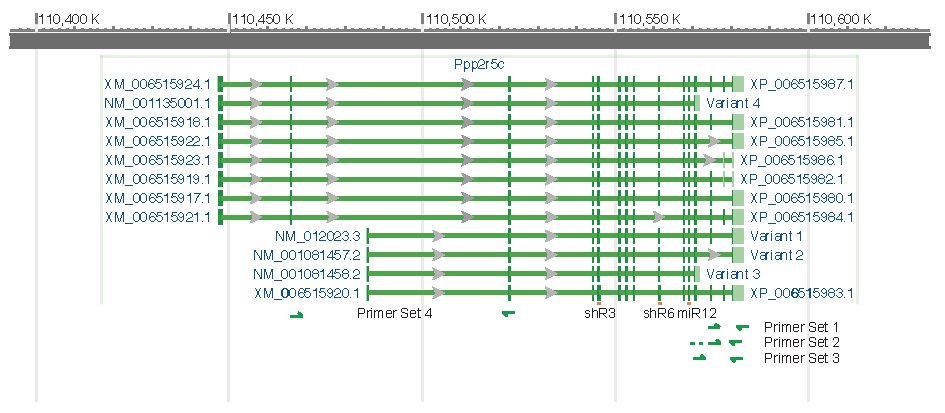
\includegraphics[width=1\textwidth]{figs/fig2-0 ppp2r5c gene structure.pdf}
\caption[Mouse PPP2R5C gene structure]{\footnotesize Mouse PPP2R5C gene structure. Four splicing isoforms, Variant 1 to 4, are displayed with exons and introns according to NCBI genbank annotation. Primer sets for Variant 1--4 are also shown in their corresponding positions. miRNAs/shRNAs targeting the common region of all isoforms, including shR3, shR6 and miR12, are also shown at their relative positions. Adapted from NCBI genbank record of mouse PPP2R5C.}
\label{fig:fig2.0}
\end{figure}

\subsection{Transcriptional change of PPP2R5C in response to metabolic state}

Since genes for metabolic regulators are often present in regulatory transcriptional feedback loops \cite{amemiya-kudo_promoter_2000}, I tested the relationship between the PPP2R5C expression and organismal nutritional status in various mice tissue samples by qPCR. Indeed, obese mice lacking the leptin receptor (\textit{db/db}) have significantly elevated levels of various PPP2R5C mRNA isoforms in the liver (Figure~\ref{fig:fig2.1}). By the \gls{ANOVA} (Analysis of Variance) analysis, at least for Variant 1, 2 and 4, there are significant increases in the transcriptional level of PPP2R5C in the \textit{db/db} mice liver comparing with the \textit{wt/wt} mice. The Variant 3 has also shown a similar trend through not significant. However, the total protein level of PPP2R5C, measured by home-made antibody (Section~\ref{sec:sec222}) for the mouse PPP2R5C, did not show a significant increase in the protein level. %This discrepancy in the mRNA and protein level of PPP2R5C further indicates the up-regulation in \textit{db/db} is a transcriptional feedback.

\begin{figure}[!tb]
\centering
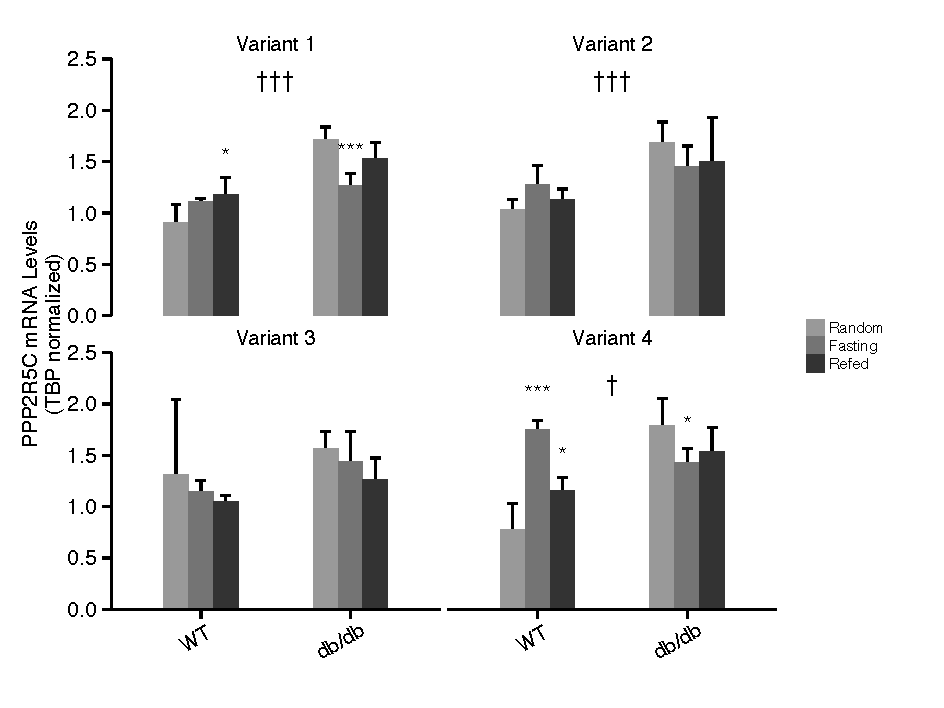
\includegraphics[width=1\textwidth]{figs/fig2-1 liver ppp2r5c.pdf}
\caption[PPP2R5C expression in the liver]{\footnotesize PPP2R5C is regulated in the mouse liver. Mouse PPP2R5C transcript variant 1--4 mRNA levels in the liver from 8-12 week C57BL/6 wild type (WT) or \textit{db/db} male mice under different nutritional statuses are shown here. Mice were fed with the normal chow diet without limit ("Random"). For "Fasting" and "Refed", mice were first starved for 16 hours and then allowed to the normal chow diet access for 6 hours. Error bar: std. dev. (this is the same for all following figures with error bars). * and *** for p-value<0.05 and 0.001 by the t-test within each mice genotype (WT or \textit{db/db}) and feeding regime (Random, Fasting, and Refed) in R. p-value was adjusted by Benjamini-Hochberg procedure in R. $\dagger$ and $\dagger\dagger\dagger$ for p-value<0.05 and 0.001 by \gls{ANOVA} analysis with comparison between wt and \textit{db/db} mice.}
\label{fig:fig2.1}
\end{figure}

Another interesting finding in the liver \gls{ppp2r5c} mRNA profile is that at least the Variant 4 in wild type mice has a transcriptional increase in response to fasting. And this response is reversed after 6-hour re-feeding. Though not significant, Variant 2 shows a similar trend. Additionally, there are also some significant changes in Variant 1 within wild type or \textit{db/db} mice between different nutritional statuses. However, these trends are not clear in other isoforms and could be isoform-specific features.


\begin{figure}[!tb]
\centering
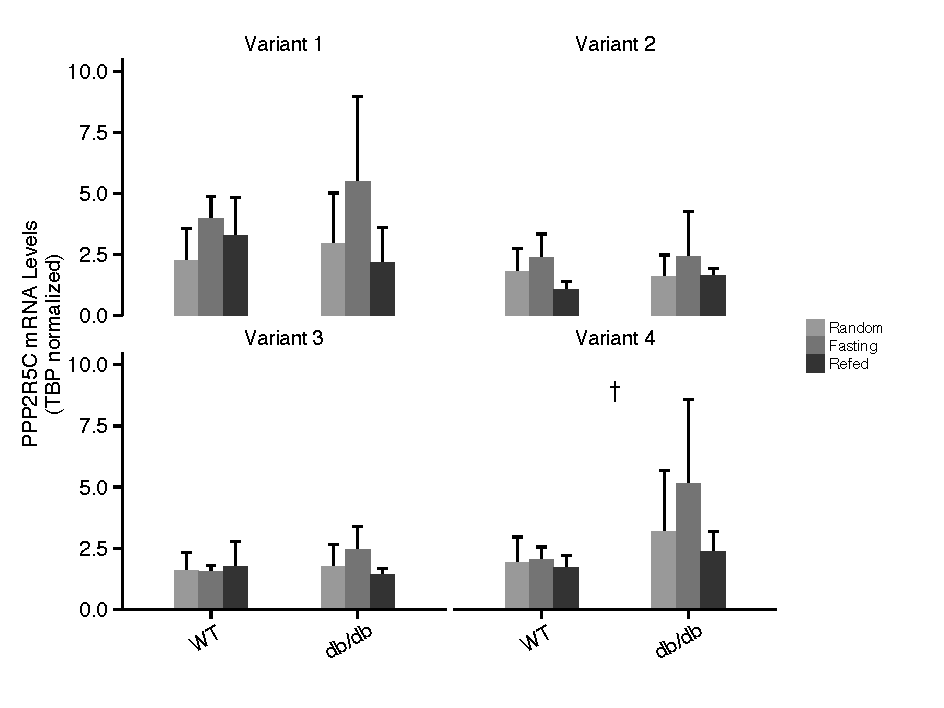
\includegraphics[width=1\textwidth]{figs/fig2-2 adipose ppp2r5c.pdf}
\caption[PPP2R5C expression in adipose tissues]{\footnotesize PPP2R5C is regulated in mouse adipose tissues. Mouse PPP2R5C transcript variant 1--4 mRNA levels in adipose tissues from 8-12 week C57BL/6 wild type or \textit{db/db} male mice under different nutritional statuses are shown here. Mice were fed with the normal chow diet without limit ("Random"). For "Fasting" and "Refed", mice were first starved for 16 hours and then allowed to the normal chow diet access for 6 hours. PPP2R5C Variant 1--4 are referenced according to NCBI. $\dagger$ for p-value<0.05 by \gls{ANOVA} analysis with comparison between wt and \textit{db/db} mice.}
\label{fig:fig2.2}
\end{figure}

In mouse abdominal white adipose tissues, there is also a significant trend in which most of \gls{ppp2r5c} variants have elevated mRNA levels in \textit{db/db} mice, especially for Variant 4 (Figure~\ref{fig:fig2.2}). There is a significant transcriptional increase in \textit{db/db} mouse adipose tissues in most nutritional statuses even with larger standard deviation compared with the liver \gls{ppp2r5c}. This phenomenon is also validated to be true in another independent qPCR analysis of mouse adipose samples, which was done by Katrin Stra{\ss}burger in our lab (data not shown). The same transcriptional change pattern shared between the liver and adipose tissue PPP2R5C indicates a similar function performed by PPP2R5C in the liver and adipose tissues. Interestingly, this match between adipose tissue and liver had also been reiterated in the liver and subcutaneous adipose tissues in healthy human controls and type 2 diabetic patients (See details in Section~\ref{sec:sec2.6}). This further indicates the conserved function of PPP2R5C between mice and human, and raises the interest to study PPP2R5C's role in metabolic diseases, such as Type 2 Diabetes. Combining the evolutionary similarity between adipose and liver (fat body in \textit{Drosophila} mimics the function of the liver and adipose tissues \cite{hietakangas_regulation_2009}), and the obese phenotype in PPP2R5C knockout mice and the fatty liver phenotype I have found after PPP2R5C knockdown in liver (Figure~\ref{fig:fig2.31}), it is reasonable to hypothesize the similar molecular function of PPP2R5C is shared by the mouse liver and adipose tissues. 

\begin{figure}[!tb]
\centering
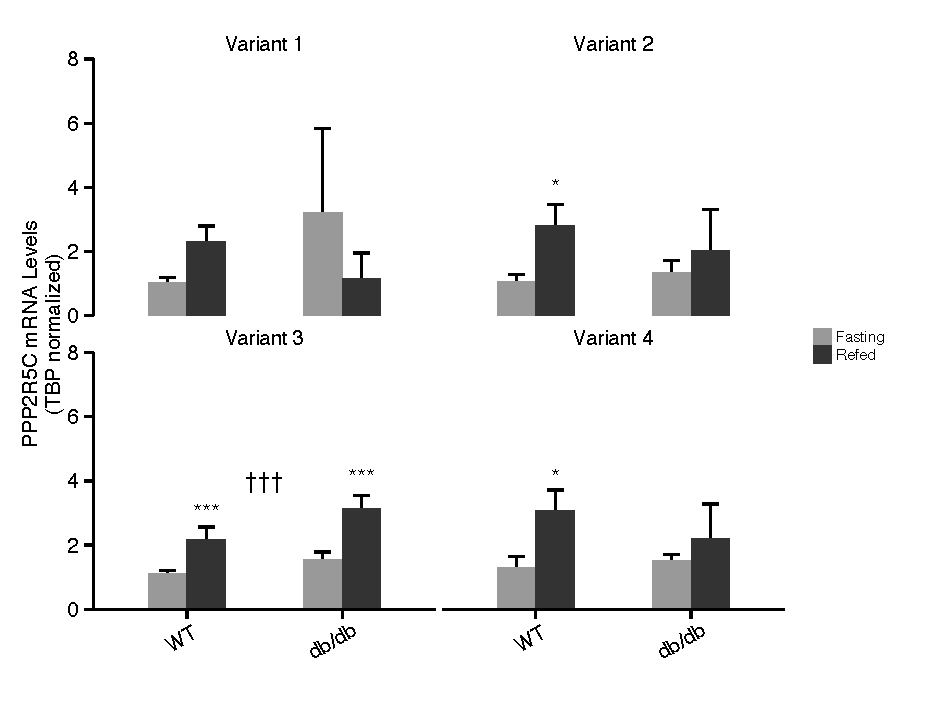
\includegraphics[width=1\textwidth]{figs/fig2-3 muscle ppp2r5c.pdf}
\caption[PPP2R5C expression in the muscle]{\footnotesize PPP2R5C is regulated in the mouse muscle. Mouse PPP2R5C transcript variant 1--4 mRNA levels in the muscle from 8-12 week C57BL/6 wildtype or \textit{db/db} male mice under different nutritional statuses are shown her. For "Fasting" and "Refed", mice were first starved for 16 hours and then allowed to the normal chow diet access for 6 hours. * and *** for p-value<0.05 and 0.001 by t-test within each mice genotype (WT or \textit{db/db}) and feeding regime (Random, Fasting, and Refed) in R. p-value was adjusted by Benjamini–Hochberg procedure in R. $\dagger\dagger\dagger$ for p-value<0.05 by \gls{ANOVA} analysis with comparison between wt and \textit{db/db} mice.}
\label{fig:fig2.3}
\end{figure}

PPP2R5C expression is nutritionally regulated in other metabolic relevant tissues such as the muscle, although in an opposite way as that for the liver and adipose tissues. In the mouse gastrocnemius muscle, PPP2R5C expression is increased upon re-feeding (Figure~\ref{fig:fig2.3}). This is significant for all variants except Variant 1, though the trend is still clear. However, this regulation is blunted in \textit{db/db}  mice compared to control mice in almost all isoforms but Variant 3. The Variant 3 in both wt and \textit{db/db} mice show an increased expression upon re-feeding. In addition, Variant 3 has also increased in \textit{db/db} mice. In comparison with the liver and adipose PPP2R5C, The opposite transcriptional response of PPP2R5C in the muscle during switch from fasting to re-feeding suggests a distinctive role of PPP2R5C in metabolically relevant tissues under different nutrient conditions.


\subsection{Transcriptional change of PPP2R5C in pathophysiology}

\begin{figure}[!tb]
\centering
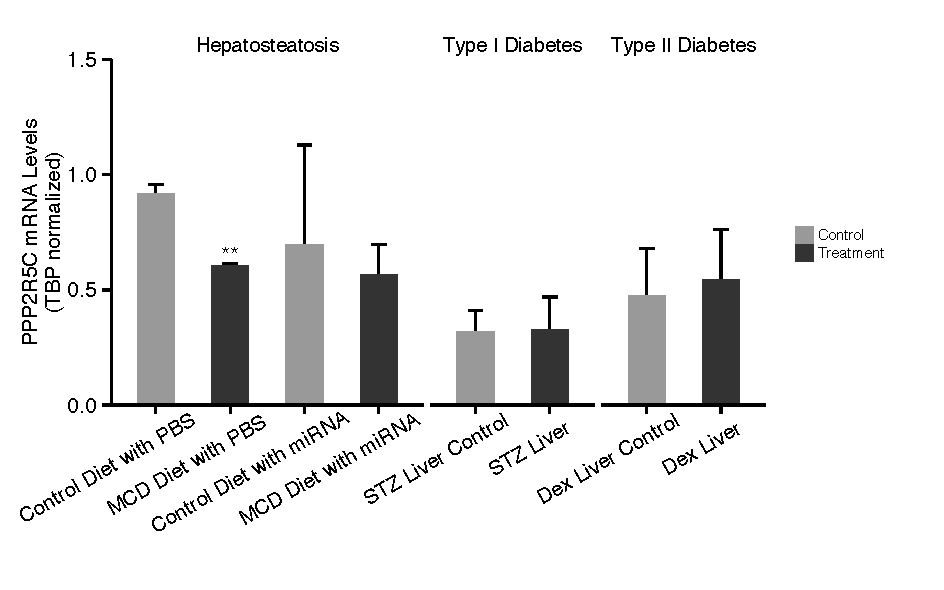
\includegraphics[width=1\textwidth]{figs/fig2-4 liver 34sample ppp2r5c.pdf}
\caption[PPP2R5C mRNA levels in Type I\&II Diabetes or Hepatosteatosis]{\footnotesize PPP2R5C transcriptional change in different pathophysiological conditions. Liver PPP2R5C mRNA levels were evaluated by qPCR in control or treatment group for the mouse model in Hepatosteatosis, Type I diabetes, and Type II diabetes. For Hepatosteatosis model, 16 week old male C57Bl6/J mice were fed with Methionine-Choline Deficient (MCD) diet or control diet for 4 weeks. In the Type I diabetes model, mice was treated with Streptozotocin (STZ) or control. For Type II diabetes model, mice was treated with Dexamethasone (Dex) or control. ** for p-value<0.01 by t-test in R.}
\label{fig:fig2.4}
\end{figure}

I have also tested PPP2R5C expression levels among various mouse models for different diseases such as Type I\&II diabetes and hepatosteatosis. The liver \gls{ppp2r5c} shows significantly reduced total mRNA level compared to control in the mouse liver from mouse hepatosteatosis model (Figure~\ref{fig:fig2.4}). However, in other disease models, there are no significant change in PPP2R5C mRNA level. In Dexamethasone induced mouse type 2 diabetes model, no strong increase in liver PPP2R5C mRNA levels shows a discrepancy with the genetic model of type 2 diabetes mouse model (\textit{db/db} in Figure~\ref{fig:fig2.1}). This difference could be due to different mechanisms for developing symptoms of type 2 diabetes in the mouse \cite{severino_low-dose_2002,king_use_2012}.  

In sum, although I have no data suggesting that these transcriptional changes have any functional relevance, these results suggest there might be links between \gls{ppp2r5c} and metabolic states or pathophysiological conditions. The transcription factor binding prediction \cite{_sabiosciences_????} on mouse PPP2R5C promoter shows several transcription factors, like \gls{nfkb} and HNF1\textalpha{}, are binding the mouse PPP2R5C promoter in ChIP assays. PPP2R5C has been shown to be involved in \gls{nfkb} pathway for T cell activation \cite{breuer_protein_2014}, and predicted \gls{nfkb} sites in PPP2R5C promoter indicate feedback regulation from \gls{nfkb} pathway. HNF1\textalpha{} has been genetically linked to maturity-onset diabetes of the young (MODY), and regulating several liver-specific gene expressions, such as albumin \cite{owen_monogenic_2013}. HNF1\textalpha{}'s potentially binding sites on PPP2R5C promoter indicate co-misregulation in diabetes.  

Although the whole body knockout mouse model for PPP2R5C showed increased adiposity \cite{varadkar_protein_2014}, distinct functions of PPP2R5C for metabolic homeostasis in a tissue-specific manner (in mammals) are widely unknown. A tissue-specific knockout or knockdown of PPP2R5C would shed more light on its functions in metabolic control. Since PPP2R5C has more than four splicing isoforms when the project was started, the primer sets 1--4 used throughout the thesis are representing more than one transcript of PPP2R5C (Figure~\ref{fig:fig2.0}). RNA sequencing for these samples would give more information about the differential regulation of various splicing isoforms.

\section{Antibody and virus preparation for PPP2R5C study}

\subsection{Selecting shRNA/miRNA for efficient knockdown of PPP2R5C}

In order to characterize the mammalian function of \gls{ppp2r5c},  I chose the mouse model  to decipher the molecular link for PPP2R5C in its potential role in metabolism. At the first step, I designed different \gls{shrna}s and \gls{mirna}s targeting common region of all PPP2R5C mRNA isoforms from online RNAi design website from Invitrogen \cite{_invitrogen_2014} (final candidates used throughout the thesis are shown in Figure~\ref{fig:fig2.0} and Table~\ref{tab:tab7}). Then I cloned shRNAs into pENTR U6, and miRNAs into pcDNA 6.2 GW EmGFP, both were purchased from Invitrogen. To have a reporter for PPP2R5C knockdown efficiency, I cloned PPP2R5C Variant 2 into 3\textsuperscript{$\prime$} UTR of renilla luciferase reporter (pRL-CMV renilla) and co-transfected with expression vectors for shRNAs and miRNAs in HEK293T cell. Knockdown efficiency was monitored for shRNAs and miRNAs as firefly luciferase normalized activity (Figure~\ref{fig:fig2.5}). 

\begin{figure}[htbp]
\centering
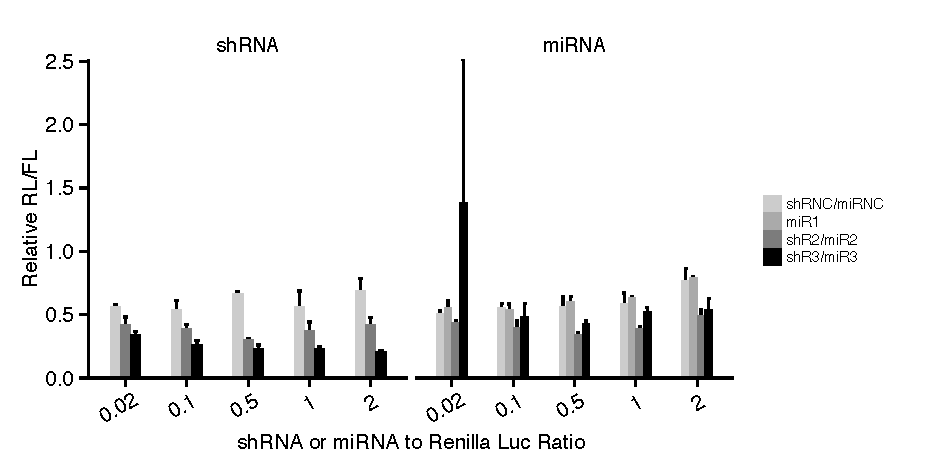
\includegraphics[width=1\textwidth]{figs/fig2-5 shR miR kd luc.pdf}
\caption[shRNA/miRNA KD efficiency on PPP2R5C luciferase reporter]{\footnotesize KD efficiency for shRNAs/miRNAs are measured on PPP2R5C variant 2 luciferase reporter. PPP2R5C variant 2 was cloned into 3\textsuperscript{$\prime$} UTR of firefly luciferase reporter (pRL-CMV renilla). RL-Var2 reporter was used to evaluated shRNA/miRNA KD efficiency via co-transfection with miRNA/shRNA expression construct at different ratios in HEK293T cell. Renilla luciferase (RL) activity was normalized against firefly luciferase (FL).}
\label{fig:fig2.5}
\end{figure}

After comparing the dynamic efficiency with different shRNAs or miRNAs to reporter plasmid ratios (Figure~\ref{fig:fig2.5}), shR3 is discovered to be the shRNA with strongest knockdown efficiency in all transfection settings with different ratios of shRNA expressing plasmid and PPP2R5C Variant 2 knockdown efficiency reporter. miR2 is the current best miRNA candidate while other two miRNAs have very mild knockdown efficiency. Furthermore, knockdown efficiency was also cross-validated by Western Blot of HA-tagged PPP2R5C Variant 2 (Figure~\ref{fig:fig2.6a}). Again, shR3 is shown to be the best shRNA candidate with almost complete knockdown at protein level when co-expressed with HA-tagged Variant 2. Thus, I chose shR3 to be the shRNA for PPP2R5C knockdown in different models, from cell to mouse. However, miRNA candidates have different performances in protein level knockdown (Figure~\ref{fig:fig2.6a}). miR3 has better knockdown efficiency than miR2 at protein level, but still has not reach the extent of shR3.

In order to achieve at least 80\% knockdown efficiency both in protein and transcription level, I did a bigger scale of searching \gls{mirna} candidate. I designed 12 new miRNAs and cloned them as before. I also performed similar Western Blot validation across various miRNAs (Figure~\ref{fig:fig2.6b}). In this experiment, miR12 was discovered to be the best miRNA against \gls{ppp2r5c} so far (only 5\% Variant 2 left comparing with control miRNA at protein level, Figure~\ref{fig:fig2.6c}), and chosen to be the miRNA for PPP2R5C knockdown \textit{in vivo}. 

\begin{figure}[htbp]
\centering

	\begin{subfigure}[t]{0.375\textwidth}
	\subcaption{shRNA/miRNA KD efficiency by western blot}
	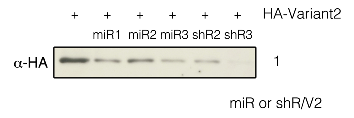
\includegraphics[width=1\textwidth]{figs/fig2-6a1.pdf}
    \label{fig:fig2.6a}
	\end{subfigure}%
          %add desired spacing between images, e. g. ~, \quad, \qquad, \hfill etc.
          %(or a blank line to force the subfigure onto a new line)
\\
	\begin{subfigure}[t]{0.625\textwidth}
	\subcaption{New set of miRNAs' KD efficiency by western blot}
	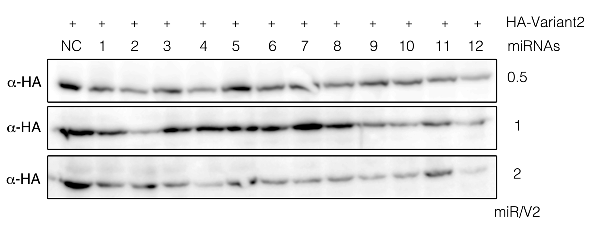
\includegraphics[width=1\textwidth]{figs/fig2-6a2.pdf}
    \label{fig:fig2.6b}
	\end{subfigure}%
          %add desired spacing between images, e. g. ~, \quad, \qquad, \hfill etc.
          %(or a blank line to force the subfigure onto a new line)
\\
	\begin{subfigure}[t]{1\textwidth}
	\subcaption{Quantification of miRNA's KD efficiency in (b)}
	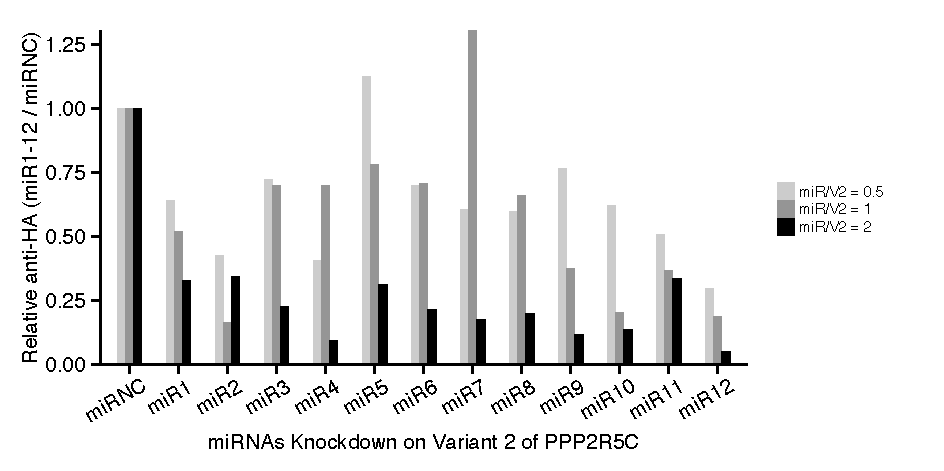
\includegraphics[width=1\textwidth]{figs/fig2-6b miR kd v2.pdf}
    \label{fig:fig2.6c}
	\end{subfigure}
\caption[shRNA/miRNA KD efficiency on PPP2R5C protein level]{\footnotesize Knockdown (KD) efficiency validated by western on PPP2R5C. (a--b) PPP2R5C KD efficiency by miRNAs and shRNAs. miRNA or shRNA construct was co-transfected with HA-tagged Variant 2 of PPP2R5C at different ratios in 293T cell. Total lysates after 3-day transfection were used to measure KD efficiency by blotting with \textalpha{}--HA antibody. (c) Quantification of miRNAs KD efficiency on PPP2R5C in Image J. }
\label{fig:fig2.6}
\end{figure}


\subsection{Generating Guinea Pig antibody for endogenous PPP2R5C detection}\label{sec:sec222}

To monitor \gls{ppp2r5c}'s endogenous regulation as well as the knockdown efficiency, I had to generate a specific antibody for mouse PPP2R5C. Although there was commercial antibody against mammalian PPP2R5C available from Abcam, I tested it and found it was failed in the specificity test, in which Variants 1--4 were over-expressed in mouse Hepa 1-6 cells to see any increased band matched with the size of PPP2R5C protein. Then I decided to make a polyclonal antibody against mouse PPP2R5C in the lab. I chose Variant 3 to be the immunizing antigen in guinea pig due to its smaller size, and potentially better solubility in bacteria than other isoforms. The recombinant Variant 3 was successfully produced in bacteria with a 6$\times$His tag. The IMAC (Immobilized metal ion Affinity Chromatography) purification gave a good amount enough for immunization (\textasciitilde1 mg). And the purity of recombinant Variant 3 was also good enough to have high specificity during antibody production (\textit{circa} 89\% in Coomassie brilliant blue staining, Figure~\ref{fig:fig2.7}). 

\begin{SCfigure} % side caption
\centering
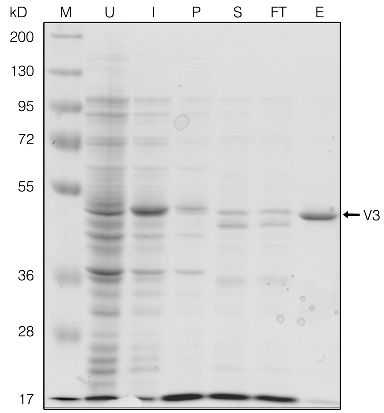
\includegraphics[width=0.5\textwidth]{figs/fig2-7 v3 purify.pdf}
\caption[Recombinant Variant 3 expression and purification]{\footnotesize PPP2R5C Variant 3 (V3) was cloned into pETM-11 (EMBL protein expression/purification facility) to be expressed in E. \textit{coli.} BL21-CodonPlus(DE3)-RIL strain. pETM-11 with V3 was electroporated into RIL and induced at 1 mM IPTG (Isopropyl \textbeta{}-D-1-thiogalactopyranoside) at 18 \celsius{} overnight. 1 mL bacteria before induction (U) and after induction (I) were taken to control the induction efficiency. Bacteria pellet after induction was lysed in lysis buffer (10mM MgCl\textsubscript{2}, 150mM NaCl, 10mM Imidazole, 20mM Tris pH 7.5) with 1 mg/ml Lysozyme, and separated into insoluble (P) and soluble fraction (S). Soluble fraction was loaded onto Ni-NTA column, and the flow-through fraction (FT) was collected. Final elute was collected in lysis buffer with 500mM Imidazole (E). All fractions from purification were run in 12\% SDS-PAGE gel with protein marker (M) and stained with GelCode Coomassie stain.}
\label{fig:fig2.7}
\end{SCfigure}

Polyclonal antibody production in guinea pig was produced with Freund's adjuvant. After 4th boosting immunization, I collected sera from guinea pig by heart puncture under animal welfare regulation in Germany, and with the generous help from Stefan F\"o{\ss}el in DKFZ's animal core facility. I tested the specificity of anti-sera for \gls{ppp2r5c} in both endogenous PPP2R5C knockdown (KD) and different PPP2R5C isoforms over-expression (Figure~\ref{fig:fig2.8}). Even at 1:5000 dilution, PPP2R5C anti-sera could still detect various PPP2R5C isoforms' over-expression and the endogenous knockdown of PPP2R5C by the adenovirus-packaged shR3 in Hepa 1-6.

\begin{figure}[htbp]
\centering
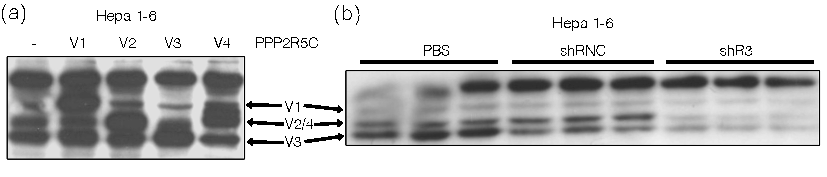
\includegraphics[width=1\textwidth]{figs/fig2-8 gp anti-v3 kd OE.pdf}
\caption[Specificity of GP antibody for PPP2R5C]{\footnotesize Antibody specificity for PPP2R5C in Hepa 1-6 lysates. (a) Variant 1--4 (V1--4) were over-expressed in Hepa 1-6 for 3 day. Total lysates from control (no over-expression) or V1--4 were submitted for Western Blotting by guinea pig antibody against PPP2R5C. V1--4 were corresponding to 3 lower bands. The most upper band could be non-specific band or other protein with high PPP2R5C homology, such as PPP2R5D. (b) knockdown efficiency on endogenous PPP2R5C by adenovirus packaged with shR3. 3 lower bands is size matched to V1--4 and showed a clear reduction in shR3. Band corresponding to V3 already showed reduction in shRNC comparing to PBS control.}
\label{fig:fig2.8}
\end{figure}

Interestingly, the adenovirus-packaged shRNC, which is a non-targeting scramble \gls{shrna}, strongly decreases the PPP2R5C protein level, especially for the band size-matched with Variant 3. And this is also true for the transcriptional level of \gls{ppp2r5c} (Figure~\ref{fig:fig2.9}). Specifically, Variant 3 mRNA level drops to around 40\% from low dosage (MOI (Multiplicity of Infection) = 10) to high dosage (MOI = 100, 200) of adenovirus infection. This indicates non-specific knockdown effect on Variant 3. It is known the adenovirus has strong immunogenic effect \cite{descamps_two_2009}. Strong immunogenicity could initiate some inflammation response which then affect the expression of PPP2R5C Variant 3. Interestingly, PPP2R5C has recently been shown to be involved in \gls{nfkb} mediated inflammation response \cite{breuer_protein_2014}. The PPP2R5C suppression upon high dose adenovirus infection suggests a feedback loop of PPP2R5C transcription in the immune response. This virus-mediated suppression of PPP2R5C could potentially controlled by \gls{nfkb} pathway on the predicted \gls{nfkb} sites in its promoter \cite{_sabiosciences_????}. 

\begin{figure}[htbp]
\centering
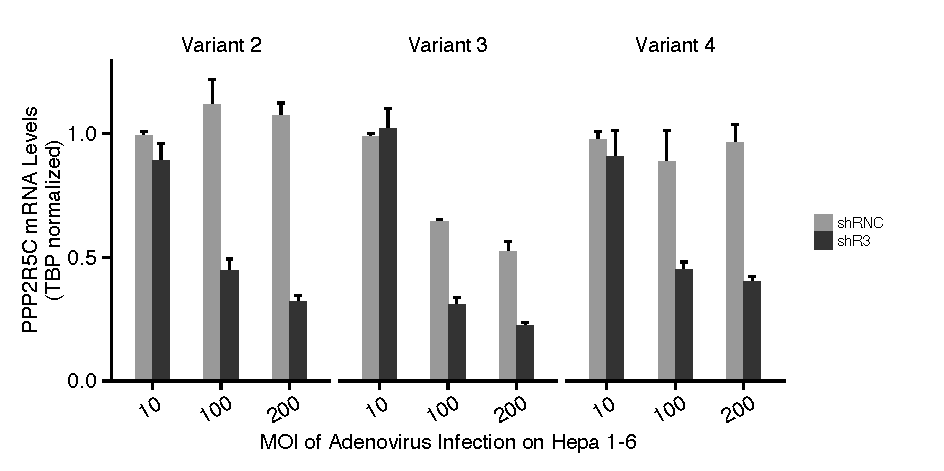
\includegraphics[width=1\textwidth]{figs/fig2-9 hepa ad kd.pdf}
\caption[Knockdown profile of endogenous PPP2R5C in Hepa 1-6]{\footnotesize Knockdown profile of endogenous PPP2R5C isoforms in Hepa 1-6 cells. Adenovirus with different \gls{moi}s (10, 100, 200) was diluted in PBS and infecting Hepa 1-6 for 3 days. The quantitative PCR analysis of PPP2R5C Variant 2/3/4 shows nice knockdown efficiency profile, which is dependent on MOI for all isoforms. MOI at 10 shows almost no reduction in mRNA level for all isoforms. MOI at 100 and 200 show a similar level of significant knockdown. Variant 3 is sensitive to control Adenovirus (shRNC) and shows a reduction in mRNA level at MOI of 100 or 200. }
\label{fig:fig2.9}
\end{figure}


\section{PPP2R5C negatively regulates glycolysis and lipogenesis}\label{sec:sec2.3}

\subsection{PPP2R5C KD in Hepa 1-6 increases glycolysis}

With efficient \textit{in vitro} knockdown tools for \gls{ppp2r5c}, I firstly studied the Hepa 1-6 to decipher the functional role of PPP2R5C, especially in metabolism control. As shown in Figure~\ref{fig:fig2.8}, endogenous PPP2R5C could be successfully knocked down at efficiency of 80\% by adenovirus-packaged shR3. After 3-day infection, mutant Hepa 1-6 cells with PPP2R5C knockdown show a clear increase in glycolysis, which is initially observed as deeper brownness of culture media in PPP2R5C KD Hepa 1-6 cells. Indeed, the glucose consumption assay (Figure~\ref{fig:fig2.10a}) indicates a strong increase in the glycolysis rate even in the last 24 hour of infection period. Accordingly, the lactate production (Figure~\ref{fig:fig2.10b}) has also similar extent of the increase as that in the glucose consumption. These pieces of evidence demonstrate that PPP2R5C could be a negative regulator of glycolysis.

\begin{figure}[htbp]
\centering
	\begin{subfigure}[t]{0.48\textwidth}
	\subcaption{Glucose consumption}
	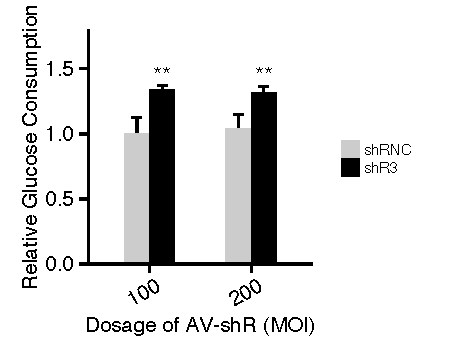
\includegraphics[width=1\textwidth]{figs/fig2-10a glucose kd.pdf}
    \label{fig:fig2.10a}
	\end{subfigure} %
~
	\begin{subfigure}[t]{0.48\textwidth}
	\subcaption{Lactate production}
	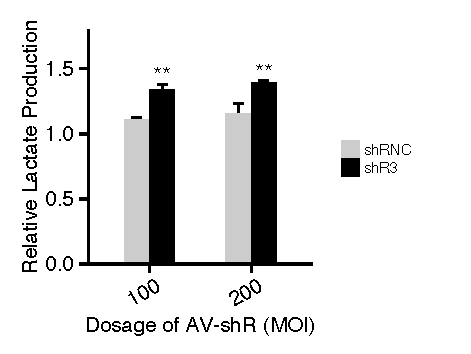
\includegraphics[width=1\textwidth]{figs/fig2-10b lactate kd.pdf}
    \label{fig:fig2.10b}
	\end{subfigure}
\caption[PPP2R5C KD increases glycolysis in Hepa 1-6]{\footnotesize PPP2R5C knockdown promotes the glucose consumption and lactate production in Hepa 1-6. Hepa 1-6 cells were infected with adenovirus packaged either with non-targeting scramble shRNA (shRNC) or PPP2R5C targeting (shR3) at \gls{moi} of 100 or 200 for 3-day knockdown. Infection was done in first 24 hours and then Hepa 1-6 cells were washed by fresh medium. The glucose consumption (a) and lactate production (b) were measured in the last 24-hour window of knockdown. They were background-subtracted from glucose and lactate concentration in fresh medium and normalized to total protein. ** for p-value<0.01 by t-test within each MOI in R.}
\label{fig:fig2.10}
\end{figure}

In addition, I also employed seahorse experiment to confirm the increased glycolysis phenotype after \gls{ppp2r5c} knockdown. When normalized to cell nuclei counting by DAPI staining, Hepa 1-6 knockdown cells have increased AUC (Area Under Curve) of glycolysis rate comparing with control adenovirus infected cells (Figure~\ref{fig:fig2.11}). The increase becomes statistically significant after oligomycin is added, which boosts the maximal glycolytic activity. Combining with data from glucose consumption and lactate production (Figure~\ref{fig:fig2.10}), it is clearly demonstrated that the PPP2R5C knockdown promotes the glucose uptake and glycolysis in Hepa 1-6 cells.

\begin{figure}[htbp]
\centering
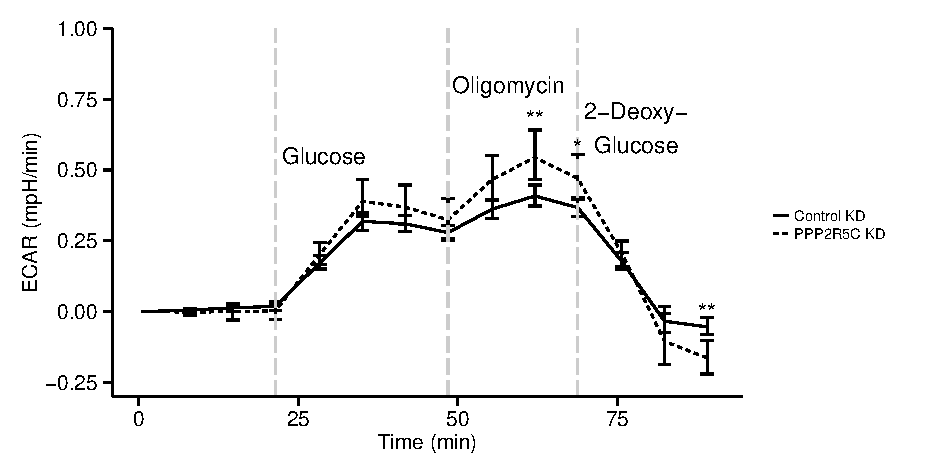
\includegraphics[width=1\textwidth]{figs/fig2-11 seahorse.pdf}
\caption[PPP2R5C KD promotes glycolysis by seahorse measurement]{\footnotesize PPP2R5C Knockdown promotes glycolysis in seahorse experiment. Adenovirus with MOI=100 was diluted in PBS and infected Hepa 1-6 for 2 days. Then infected Hepa 1-6 was digested with trypsin from the culture plate and re-plated in 96-well plate with balanced cell number between different groups (Control KD for shRNC, and PPP2R5C KD for shR3). Glycolysis activity was measured on seahorse instrument with glycolysis stress kit. Glucose, oligomycin and 2-Deoxy-Glucose were added at the time of vertical dashed line according to the protocol in the kit. The extracellular acidification rate (ECAR, mpH/min) was recorded as an indirect readout for intracellular glycolysis rate. * and ** for p-value<0.05 and 0.01 by Wilcoxon signed-rank test.}
\label{fig:fig2.11}
\end{figure}

\subsection{PPP2R5C KD promotes glucose uptake rate in Hepa 1-6}

Although \gls{ppp2r5c} is shown to be a negative regulator of glycolysis, it is still not clear the increased glucose consumption is due to increased cell number with the same glucose uptake rate or increased glucose uptake rate within the same number of cells. On one hand, the total protein content after PPP2R5C knockdown has not changed between control and PPP2R5C knockdown cells (data not shown), which indicates no strong increase in cell proliferation. On other hand, I employed a short-term glucose uptake assay to assess the glucose uptake activity of Hepa 1-6 by measuring \gls{2nbdg} uptake in 20 min via \gls{facs} (\cref{fig:fig2.12,fig:fig2.13,fig:fig2.14}), in order to eliminate any glucose uptake effect from increasing cell number during assay time in Figure~\ref{fig:fig2.10a}. 2NBDG is a fluorescent 2-deoxyglucose analog which was widely used to monitor glucose uptake rate \cite{zou_2-nbdg_2005,nitin_molecular_2009,oneil_uptake_2005,zhong_histone_2010,kawauchi_p53_2008}.

\begin{figure}[!tbp]
\centering
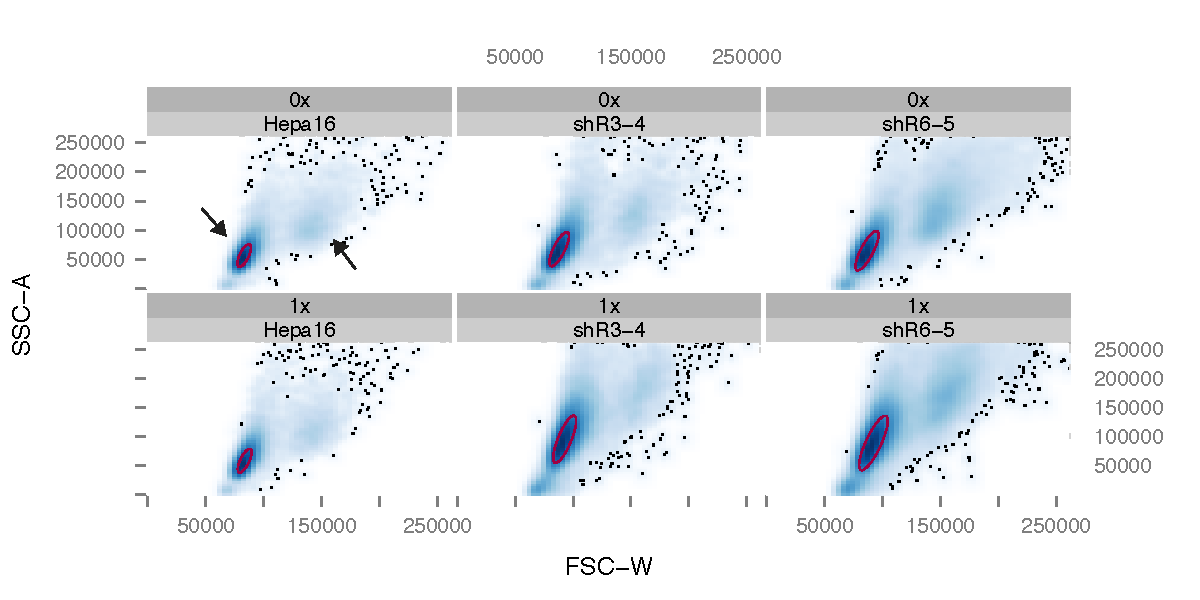
\includegraphics[width=1\textwidth]{figs/fig2-12 facs filter new.pdf}
\caption[FACS filtering for single live Hepa 1-6 cell]{\footnotesize Single live Hepa 1-6 cell filtering in FACS by R. X-coordinate is marker for cell size (FSC-W, \textbf{F}oward-\textbf{S}cattered \textbf{W}idth), and y-coordinate is cell granularity (SSC-A, \textbf{S}ide-\textbf{S}cattered \textbf{A}rea). Hepa 1-6 with stable shRNAs (shR3 or shR6) or not were induced at 30 $\mu$g/mL cumate (1x, 0x for DMSO control) for 3 day and then starved in serum-free DMEM overnight. shR3-4 and shR6-5 were single clone for shR3 and shR6. Then these cells were sensitized in KRPH (Krebs-Ringer-Phosphate-HEPES) buffer for 1 hour and followed by 20 min incubation with 100 $\mu$M 2NBDG. Finally, Hepa 1-6 cells were digested with trypsin for 3 minutes and subjected to FACS analysis. Single live Hepa 1-6 cells were clustered in FSC-SSC scatter plot and filtered out in R by using package flowCore (indicated by red circle on scatter plot). Single live cell population and doublet Hepa 1-6 cells are pointed with arrows. }
\label{fig:fig2.12}
\end{figure}

\begin{SCfigure}
\centering
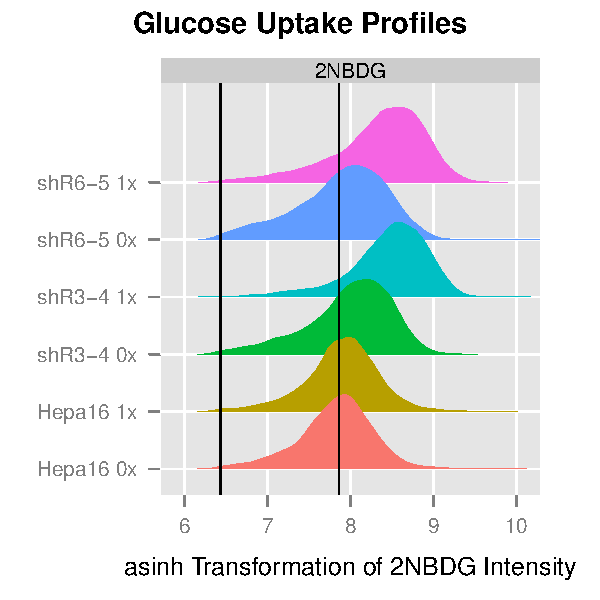
\includegraphics[width=0.5\textwidth]{figs/fig2-13 density 2NBDG.pdf}
\caption[Density plot of 2NBDG+ Hepa 1-6]{\footnotesize Density plot of Hepa 1-6 cell with positive 2NBDG uptake. Filtered single live Hepa 1-6 cells were compared for 2NBDG fluorescence intensity between Hepa 1-6 cell with 2NBDG incubation and the one without 2NBDG incubation to calculate a threshold for 2NBDG uptake (left vertical line). Median intensity in Hepa 1-6 without cumate induction (right vertical line) was calculated for better comparison between different cell lines. shR3-4 and shR6-5 were single clone for shR3 and shR6. 0x and 1x were DMSO control and 30 $\mu$g/mL cumate induction for 3 days. The fluorescence intensity was \textit{asinh} transformed to have a nice representation of intensity at different magnitudes.}
\label{fig:fig2.13}
\end{SCfigure}

Additionally, I cloned 2 sets of \gls{shrna}s (shR3 and shR6)  into a miR30-based inducible shRNA expression vector \cite{fellmann_functional_2011,_piggybac_????}, and stable Hepa 1-6 cell lines harboring genome-integrated inducible shR3 or shR6 were generated after puromycin selection. The stable inducible cell lines were used as cross-validation for results from the adenovirus-packaged shR3, and supposed to eliminate any potential virus-mediated effects given the fact of high immunogenicity of adenovirus and non-specific down-regulation on Variant 3 of PPP2R5C by adenovirus. The shR3 and shR6 expression were induced by 30$\mu$g/mL cumate for 3--4 days to achieve similar extent of knockdown efficiency as that in the adenovirus packaged shR3.

I analyzed all the data from FACS either in flowCore \cite{ellis_flowcore:_????}, flowStats \cite{hahne_flowstats:_????} and flowViz \cite{ellis_flowviz:_????} package in R, and validated the analysis again in FlowJo. There are mainly two populations in all cell lines  based on the size distribution (from empty Hepa 1-6 to two stable inducible \gls{shrna} cell lines) (Figure~\ref{fig:fig2.12}). And these two populations have not changed after shRNA expression by induction with 30 $\mu$g/mL cumate, which indicates no significant cell morphological change after \gls{ppp2r5c} knockdown. Based on particle size (FSC), it is clear that the population at the left is single live cells, and the population on the right is doublet Hepa 1-6 cells potentially from incomplete digestion by trypsin. For accurate single cell glucose uptake measurement, I chose the single live cell population for glucose uptake assay by FACS.

\begin{figure}[htbp]
\centering
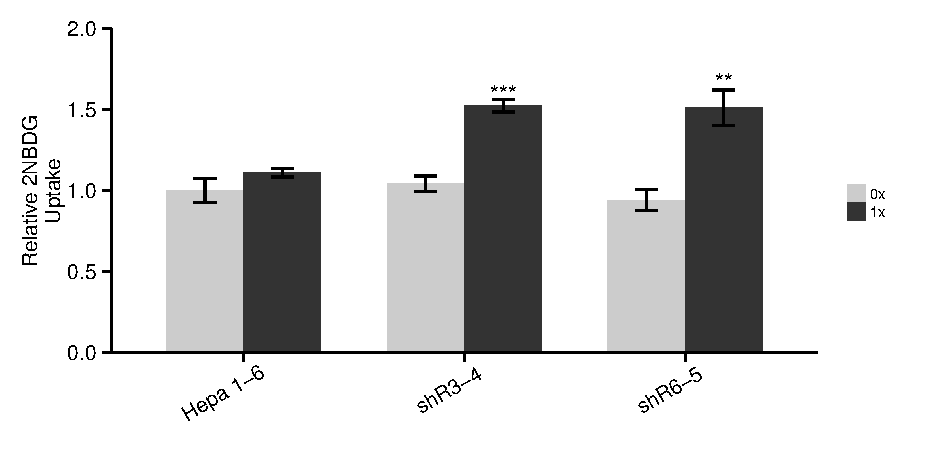
\includegraphics[width=1\textwidth]{figs/fig2-14 facs glucose uptake.pdf}
\caption[Relative quantification of 2NBDG uptake upon PPP2R5C KD]{\footnotesize 2NBDG uptake in Hepa 1-6 upon PPP2R5C knockdown. FACS data for 2NBDG uptake in empty Hepa 1-6, Hepa 1-6 with inducible shR3 and 6 (single clone shR3-4 and shR6-5) were induced at DMSO (0x) or 30 $\mu$g/mL cumate (1x) and analyzed as described in Figure~\ref{fig:fig2.13} and Figure~\ref{fig:fig2.12}. ** and *** for p-value<0.01 and 0.001 by t-test in R. }
\label{fig:fig2.14}
\end{figure}

In the first step, single live Hepa 1-6 cells were filtered out based on size (red circled area in Figure~\ref{fig:fig2.12}) with a 2D-normal distributed contour from flowCore package. Then, single live Hepa 1-6 cells were analyzed to calculate the proportion of 2NBDG positive staining with 2NBDG un-stained Hepa 1-6 cells as negative staining control. From the \textit{asinh} transformed density map of all 2NBDG positive staining, there is a obvious red-shift in the density map after \gls{ppp2r5c} knockdown (Figure~\ref{fig:fig2.13}), and almost all single live Hepa 1-6 cells have positive 2NBDG uptake. For empty Hepa 1-6 cells, there is no red-shift in density map after the cumate induction. These data clearly show that PPP2R5C knockdown could increase glucose uptake even in very short time period, such as 20 minutes. The quantification of median fluorescence intensity (MFI) is normalized and showed in Figure~\ref{fig:fig2.14}. The same phenotype has also been observed in a third independent shRNA for PPP2R5C (shR8, data not shown). 

\begin{figure}[htbp]
\centering
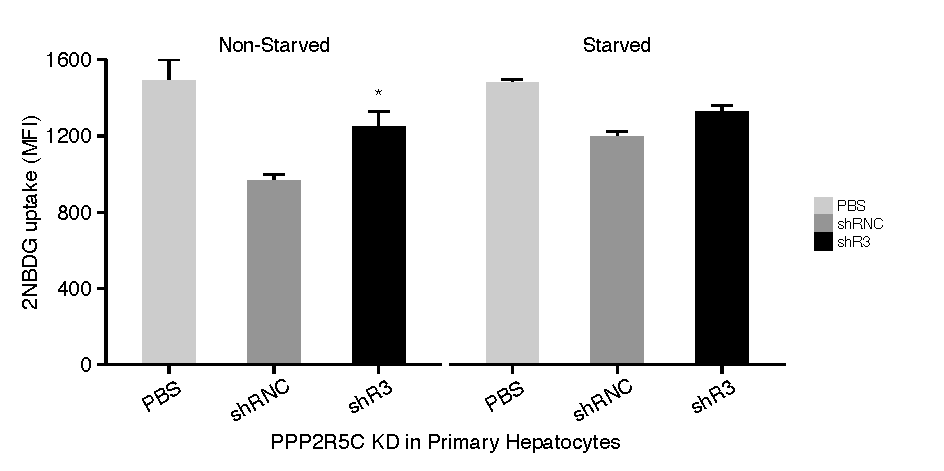
\includegraphics[width=1\textwidth]{figs/fig2-15 1st hepa glucose uptake facs.pdf}
\caption[2NBDG uptake in primary hepatocytes]{\footnotesize 2NBDG uptake in mouse primary hepatocytes upon PPP2R5C knockdown by the adenovirus with shRNC or shR3. FACS data were collected and analyzed as described in Figure~\ref{fig:fig2.14}. * for p-value<0.05 by t-test in R. n=3.}
\label{fig:fig2.15}
\end{figure}

In mouse primary hepatocytes, there is also a nice cross-validation of glucose uptake phenotype observed in Hepa 1-6 cells (Figure~\ref{fig:fig2.15}). At two different nutritional statuses, either starved for serum or non-starved, the glucose uptake, which is determined by FACS measurement of 2NBDG uptake as that in Figure~\ref{fig:fig2.14}, shows clear trend of increase in \gls{ppp2r5c} knockdown cells comparing with non-targeting \gls{shrna} control cells. For non-starved condition, the increase is statistically significant. Again, the non-targeting shRNA control adenovirus still has some non-specific virus effect on glucose uptake comparing with PBS control.

\subsection{PPP2R5C deficiency promotes \textit{de novo} lipogenesis}

Another interesting phenotype by \gls{ppp2r5c} knockdown is the increased lipid storage in the cultured primary hepatocytes (Figure~\ref{fig:fig2.16}). For cultivated mouse primary hepatocytes, I have received two sources of them, from Prof. Herzig's and Prof. Klingm\"uller's lab especially. These two sources of hepatocytes were prepared in their corresponding lab with the same protocol of isolation. However, hepatocytes from Prof. Klingm\"uller's lab were additionally counted for living cell by trypan blue staining. With these two different sources of mouse primary hepatocytes, the PPP2R5C knockdown via adenovirus-packaged shR3 shows a significant increase (approximately 2-fold) in the triglyceride storage comparing to the non-targeting shRNC or PBS control. Although relative extent of lipid storage increase is proportionally augmented with the duration of knockdown, prolonged \textit{in vitro} cultivation of primary hepatocytes sometimes ended up with de-differentiation of the hepatocyte. The de-differentiated primary hepatocytes usually show distorted and shrunken cell shape. The lipid storage increase phenotype could not be observed under this condition, such as 3-day adenovirus infected hepatocytes from Prof. Herzig's Lab at DKFZ ("Herzig 3 Day" in Figure~\ref{fig:fig2.16}). 

\begin{figure}[htbp]
\centering
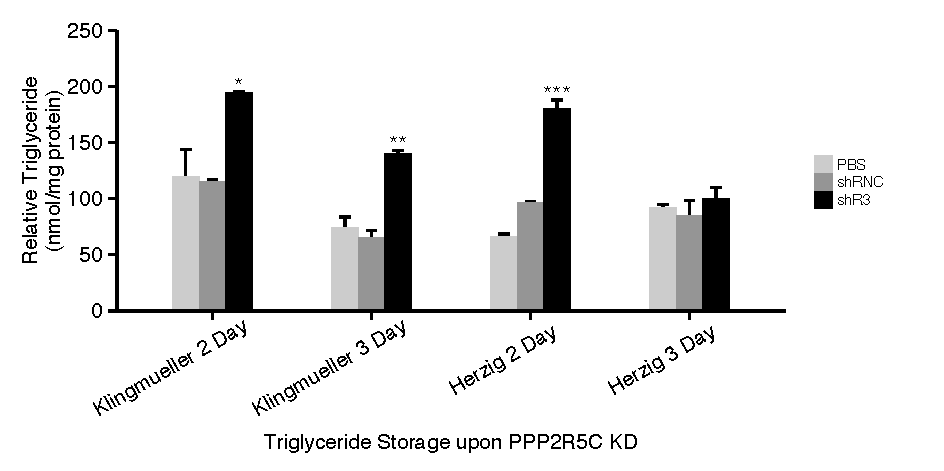
\includegraphics[width=1\textwidth]{figs/fig2-16 1st hepa tag.pdf}
\caption[Triglyceride in primary hepatocytes upon PPP2R5C KD]{\footnotesize PPP2R5C knockdown increases lipid storage in primary hepatocytes. Primary hepatocytes were infected with adenovirus at the same condition as in Figure~\ref{fig:fig2.15}. Lipid fraction was extracted by methanol-chloroform method \cite{folch_simple_1957} and measured for free glycerol released from lipase digestion.  *, ** and *** for p-value<0.05, 0.01 and 0.001 by t-test in R, n=3.}
\label{fig:fig2.16}
\end{figure}

In contrary to the shRNC effect on glycolysis phenotype, the non-targeting scramble \gls{shrna} showed no effect on the lipid storage when that was comparing with PBS control. This discrepancy possibly implied complex and different mechanisms in changing glycolysis and lipid storage after \gls{ppp2r5c} knockdown. 

\begin{figure}[htbp]
\centering
	\begin{subfigure}[t]{0.48\textwidth}
	\subcaption{ATP Level}
	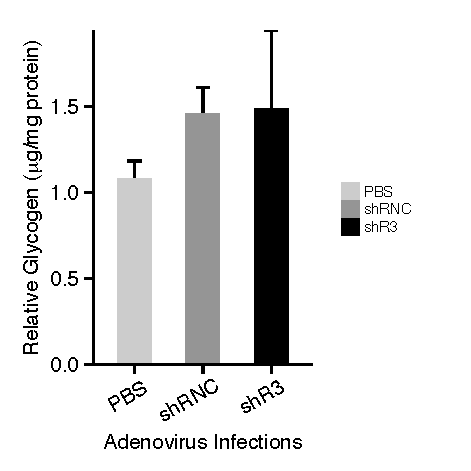
\includegraphics[width=1\textwidth]{figs/fig2-17a 1st hepa glycogen.pdf}
    \label{fig:fig2.17a}
	\end{subfigure} %
~
	\begin{subfigure}[t]{0.48\textwidth}
	\subcaption{Glycogen Storage}
	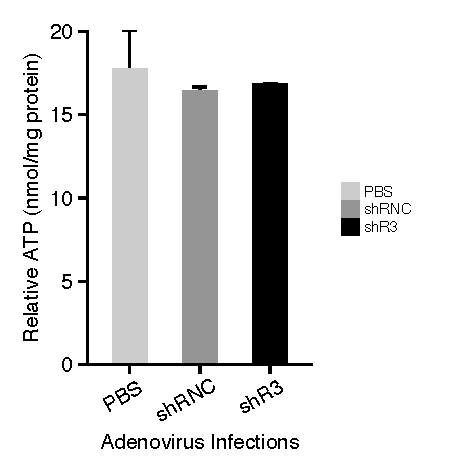
\includegraphics[width=1\textwidth]{figs/fig2-17b 1st hepa atp.pdf}
    \label{fig:fig2.17b}
	\end{subfigure}
\caption[PPP2R5C KD has no effect on ATP and Glycogen in 1\textsuperscript{o} Hepatocytes]{\footnotesize PPP2R5C knockdown does not change the ATP level (a) or the glycogen storage (b) in mouse primary hepatocytes. Primary hepatocytes were infected with the adenovirus at the same condition as in Figure~\ref{fig:fig2.14}. n=3.}
\label{fig:fig2.17}
\end{figure}

In addition to the lipid storage and glycolysis phenotype, the PPP2R5C knockdown in primary hepatocyte has no effect on the \gls{ATP} level (Figure~\ref{fig:fig2.17a}) and glycogen level (Figure~\ref{fig:fig2.17b}). This indicates the excessive energy from the increased glucose uptake is shunted into the energy storage as triglyceride storage, but not as the \gls{ATP} or glycogen in cultivated primary hepatocytes. 

\begin{figure}[htbp]
\centering
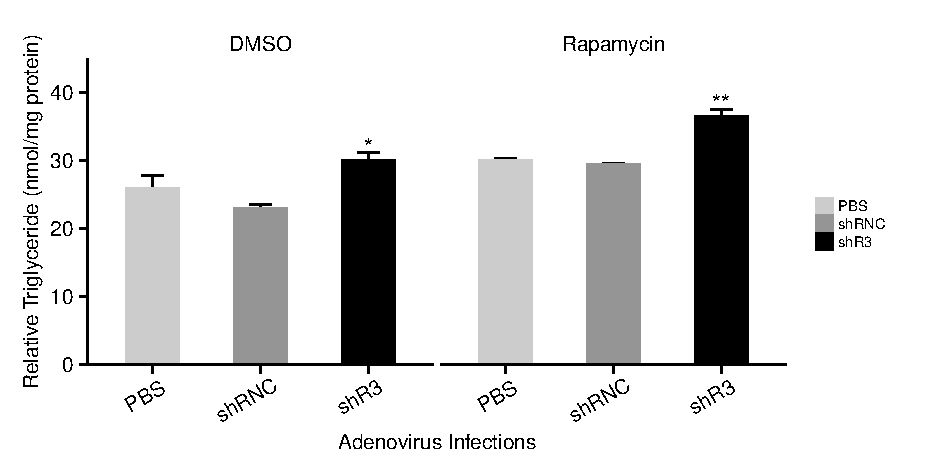
\includegraphics[width=1\textwidth]{figs/fig2-18 hepa tag rapamycin.pdf}
\caption[Triglyceride increases in Hepa 1-6 upon PPP2R5C KD]{\footnotesize PPP2R5C knockdown increases lipid storage in Hepa 1-6 independently of mTOR. Hepa 1-6 were infected with adenovirus at the same condition as in Figure~\ref{fig:fig2.10}. Lipid fraction was extracted by methanol-chloroform method and measured for free glycerol released from lipase digestion.  *, ** for p-value<0.05, 0.01 by t-test in R, n=3.}
\label{fig:fig2.18}
\end{figure}

Moreover, the lipid storage phenotype in \gls{ppp2r5c} knockdown is also conserved in another cell type, Hepa 1-6 cells (Figure~\ref{fig:fig2.18}). Even treated with \gls{mtor} inhibitor rapamycin, the lipid storage phenotype is still present without compromising its increase. This evidence indicates the mechanism how PPP2R5C affect lipid storage is either at the downstream of \gls{mtor} or in parallel with \gls{mtor}. It has been shown that the mTORC1 activation leads to the increase in glycolysis and lipogenesis via the  downstream activation of HIF1\textalpha{} and SREBP-1 \cite{duvel_activation_2010}. The increased glycolysis and lipogenesis in PPP2R5C knockdown is a phenocopy for the mTORC1 activation. 

\begin{figure}[!tb]
\centering
	\begin{subfigure}[t]{0.48\textwidth}
	\subcaption{Free Fatty Acid Uptake}
	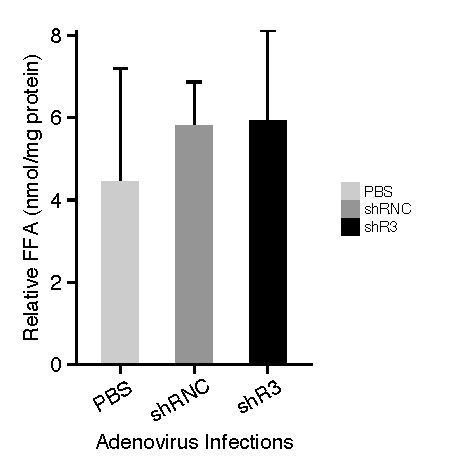
\includegraphics[width=1\textwidth]{figs/fig2-19a hepa ffa uptake.pdf}
    \label{fig:fig2.19a}
	\end{subfigure} %
~
	\begin{subfigure}[t]{0.48\textwidth}
	\subcaption{Intracellular Steady-state Free Fatty Acid}
	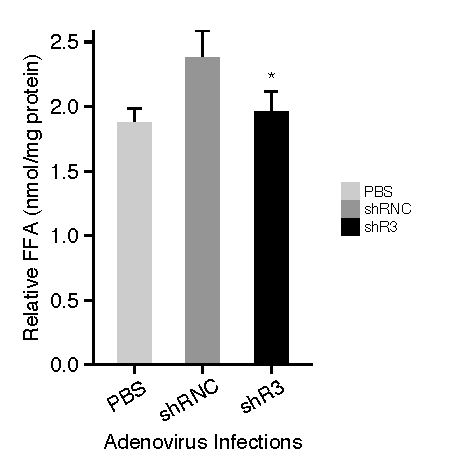
\includegraphics[width=1\textwidth]{figs/fig2-19b hepa ffa intracellular.pdf}
    \label{fig:fig2.19b}
	\end{subfigure}
\caption[Free Fatty Acid uptake is not responsible for increased triglyceride]{\footnotesize Free fatty acid in culture medium is not responsible for increased triglyceride storage inside Hepa 1-6. (a) Free fatty acid from culture media was enriched by methanol-chloroform method \cite{folch_simple_1957} and uptake was calculated from the difference in free fatty acid between fresh medium and medium after 3-day culturing. (b) Intracellular free fatty acid level. Hepa 1-6 cells were infected with adenovirus at the same condition as in Figure~\ref{fig:fig2.14}. * for p-value<0.05 by t-test in R, n=3.}
\label{fig:fig2.19}
\end{figure}

In order to further clarify the lipid storage phenotype is a result of the increased \textit{de novo} lipogenesis but not the re-esterification of absorbed free fatty acids, I measured the free fatty acid uptake from culture media and the intracellular free fatty acid in Hepa 1-6 cells upon \gls{ppp2r5c} knockdown (Figure~\ref{fig:fig2.19}). Neither of them is increased after PPP2R5C knockdown. No increase in free fatty acid uptake suggests the accumulated lipid storage could come from \textit{de novo} lipogenesis. If comparing the relative concentration of free fatty acid uptake during 3-day infection with that for fatty acid equivalent increment in triglyceride after PPP2R5C knockdown (approximately comparing 6 nmol/(mg protein) with 30 nmol/(mg protein), 1 molecule of triglyceride consists of 3 molecules of fatty acid), it is very unlikely that the increased triglyceride storage phenotype comes from the increased re-esterification of absorbed free fatty acids, but rather from \textit{de novo} biosynthesis. Also, the slight decrease in the intracellular free fatty acid concentration after PPP2R5C implies a higher flux from intracellular free fatty acid toward triglyceride synthesis when comparing with shRNC.


\section{PPP2R5C \textit{in vivo} knockdown promotes glucose uptake, triglyceride synthesis}

It was interesting to know the \gls{ppp2r5c}'s role in a cellular model, such as the Hepa 1-6 or mouse primary hepatocyte (Section~\ref{sec:sec2.3}). Data in cell culture suggested PPP2R5C's potential role in metabolism is shunting the absorbed glucose into lipid storage in a cell-autonomous fashion. But it was always more physiological-relevant when investigating the PPP2R5C's function in metabolism \textit{in vivo}. To achieve this purpose, I employed adeno-associated virus (AAV) to specifically express the \gls{mirna} targeting PPP2R5C (miR12, see Figure~\ref{fig:fig2.0} and Table~\ref{tab:tab7}) in the mouse liver and perform a long-term knockdown \textit{in vivo} as described \cite{kulozik_hepatic_2011}. Previously, the miR12 was selected as miRNA candidate based on its highest efficiency in knockdown tested in HEK293T cell (Figure~\ref{fig:fig2.6c}). The \gls{AAV} packaged miR12 was produced from Vector Biolabs (Philadelphia, USA) due to the  insufficient in-house virus production yield. I performed a pilot mouse experiment  to evaluate the \textit{in vivo} knockdown efficiency in the mouse liver. From the qPCR analysis of total PPP2R5C mRNA (Figure~\ref{fig:fig2.20a}) and protein level (Figure~\ref{fig:fig2.20b}), there is a strong reduction in both transcriptional and protein level. This AAV packaged miR12 gave me the appropriate tool to have a liver-specific manipulation of the mouse PPP2R5C. 

\begin{figure}[htbp]
\centering
	\begin{subfigure}[t]{0.48\textwidth}
	\subcaption{Knockdown efficiency by qPCR}
	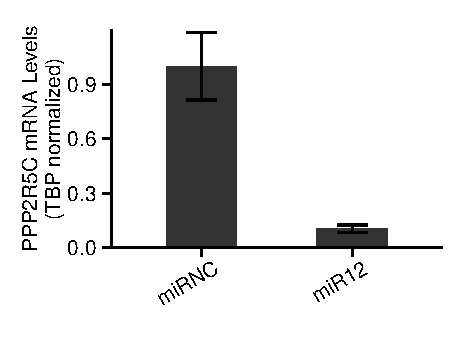
\includegraphics[width=1\textwidth]{figs/fig2-20a pilot qPCR.pdf}
    \label{fig:fig2.20a}
	\end{subfigure} %
~
	\begin{subfigure}[t]{0.48\textwidth}
	\subcaption{Knockdown efficiency in protein level}
	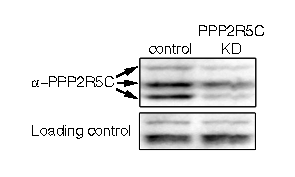
\includegraphics[width=1\textwidth]{figs/fig2-20b kd in vivo protein.pdf}
    \label{fig:fig2.20b}
	\end{subfigure}
\caption[KD efficiency for miR12 \textit{in vivo}]{\footnotesize PPP2R5C knockdown efficiency in vivo. (a) miR12's \textit{in vivo} knockdown efficiency was compared with the non-targeting control miRNC after 2 week AAV injection. qPCR was performed with the probe set for total mRNA of PPP2R5C in the liver. (b) Knockdown efficiency was evaluated at protein level. The liver endogenous PPP2R5C was detected by the home-made guinea pig antibody against it. Non-specific binding band was showed at bottom as the loading control. n=5 for qPCR analysis.}
\label{fig:fig2.20}
\end{figure}

\subsection{PPP2R5C knockdown has no impact on animal health}

With the knowledge of miR12's \textit{in vivo} knockdown efficiency, I performed another mouse experiment with longer AAV infection in order to see the relatively long term effect of PPP2R5C in metabolism. With 7 weeks of \gls{ppp2r5c} knockdown in the mouse liver, there is no severe side effect from \gls{AAV} infection, which could be demonstrated by the low level of serum \gls{alt} level and no further increase in knockdown mice (Figure~\ref{fig:fig2.21}). ALT is an enzyme mainly expressed in the liver, much less expressed in kidney, heart, muscle. The serum ALT level is normally low, and only become high when the liver is damaged or diseased (leakage across damaged hepatic cell membrane). Serum ALT level around 20 U/L was much lower than that from mice suffering liver injury (several hundred to even thunsands U/L \cite{masaki_role_2005}). 

\begin{figure}[htbp]
\centering
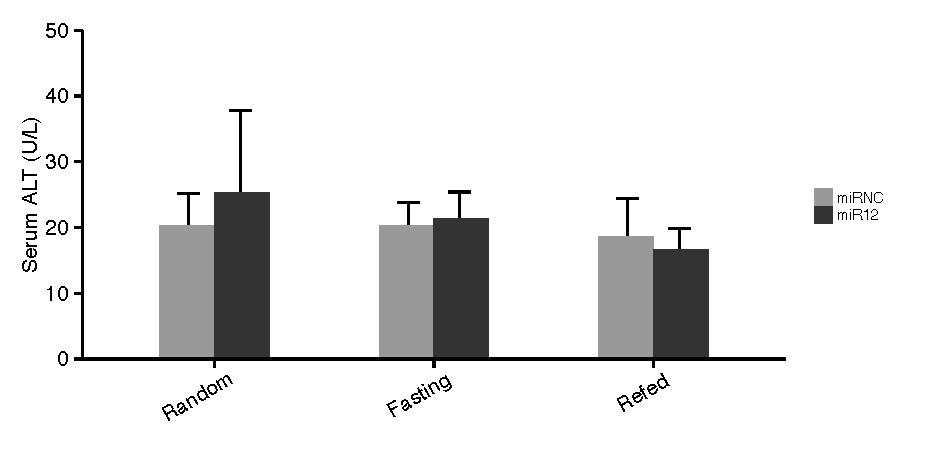
\includegraphics[width=1\textwidth]{figs/fig2-21 serum ALT.pdf}
\caption[Serum ALT after PPP2R5C KD]{\footnotesize Serum ALT (Alanine Aminotransferase) level indicates no liver injury. 8-10 week CL57BL/6 male mice were injected with adeno-associated virus packaged \gls{mirna} against mouse PPP2R5C (miR12) or scramble miRNA (miRNC) at 1$\times$10\textsuperscript{11} viral particles/mouse via tail injection in 100 $\mu$L PBS. And injected mice was sacrificed after 7-week knockdown. Before sacrificing, mice were divided into different groups for various treatments, including \textit{ad libitum} fed (Random), 16 hour fasting (Fasting), and 16 hour fasting followed by 6 hour feeding (Refed). 5 $\mu$L serum was used to measure ALT enzymatic activity. n=5 or 6.}
\label{fig:fig2.21}
\end{figure}

During the \gls{AAV} infection, mice from control and knockdown group (miRNC vs miR12) have also no significant difference in the body weight growing profile (Figure~\ref{fig:fig2.22}), which indicates no strong whole body growth change after the liver-specific PPP2R5C KD. Furthermore, I have also performed the body composition analysis  in these mice every 2 or 3 week by using echoMRI measurement. There is also no significant difference in fat (Figure~\ref{fig:fig2.22}) and lean mass (data not shown) profile between control and knockdown group. Although these mice subjected into fasting before final preparation show some difference before virus injection, and the difference remained constant during knockdown and contributed to the overall baseline difference in control and knockdown group. After sacrificing, I also measured the mouse abdominal white adipose tissue weight (Figure~\ref{fig:fig2.25}). There is also no change in abdominal white adipose tissue weight upon PPP2R5C KD. In summary, 7-week liver-specific PPP2R5C knockdown via \gls{AAV} infection has no significant morphological changes to the size of tissues or to the whole body.

\begin{figure}[htbp]
\centering
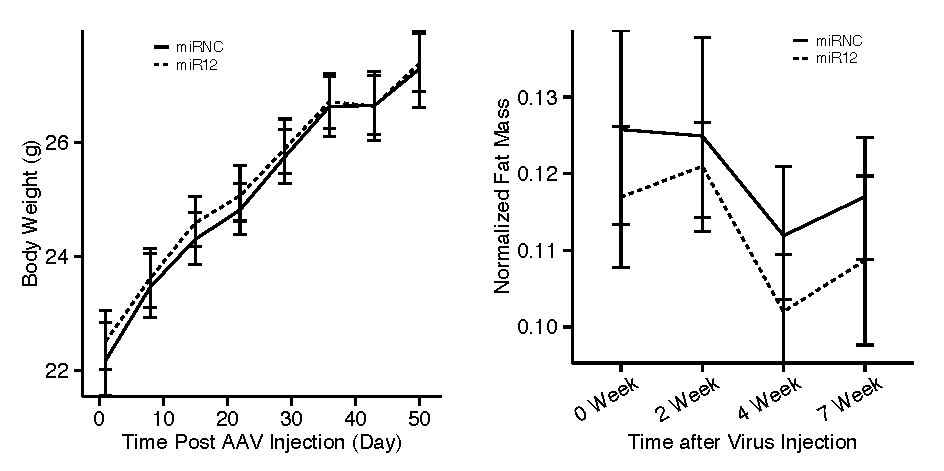
\includegraphics[width=1\textwidth]{figs/fig2-22 body weight and echoMRI fat.pdf}
\caption[Body weight and fat composition change after PPP2R5C KD]{\footnotesize Body weight and fat composition profile have no change after PPP2R5C knockdown. Mice in Figure~\ref{fig:fig2.21} were measured for body weight at each week (left panel). Time 0 was the body weight before virus injection. Whole body fat composition was calculated from fat content normalized to body weight at each time point (right panel). Week 0 indicated fat composition before virus injection. n=5 or 6.}
\label{fig:fig2.22}
\end{figure}

%\begin{figure}[htbp]
%\centering
%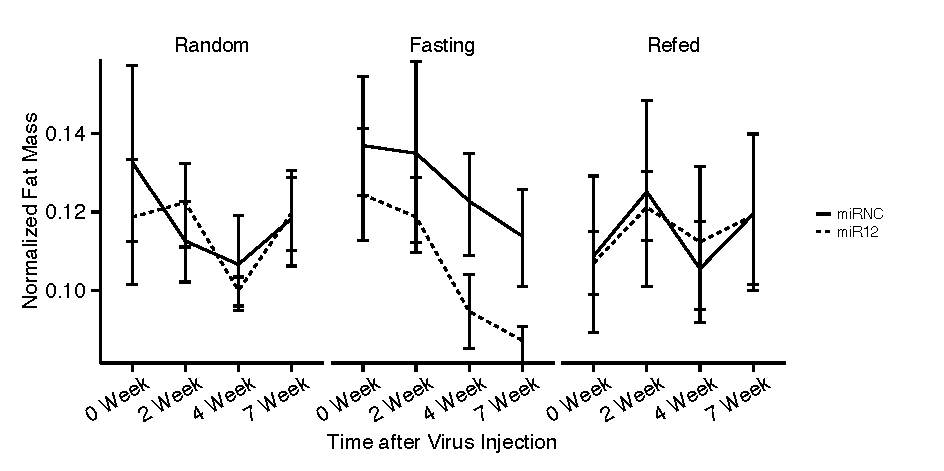
\includegraphics[width=1\textwidth]{figs/fig2-23 echoMRI fat.pdf}
%\caption[Body fat content profile after PPP2R5C KD]{\footnotesize Body fat content profile has no change after PPP2R5C knockdown. Mice were the same as Figure~\ref{fig:fig2.21}. Whole body fat composition was calculated from fat content normalized to body weight at each time point. Week 0 indicated fat composition before virus injection. n=5 or 6}
%\label{fig:fig2.23}
%\end{figure}

%\begin{figure}[htbp]
%\centering
%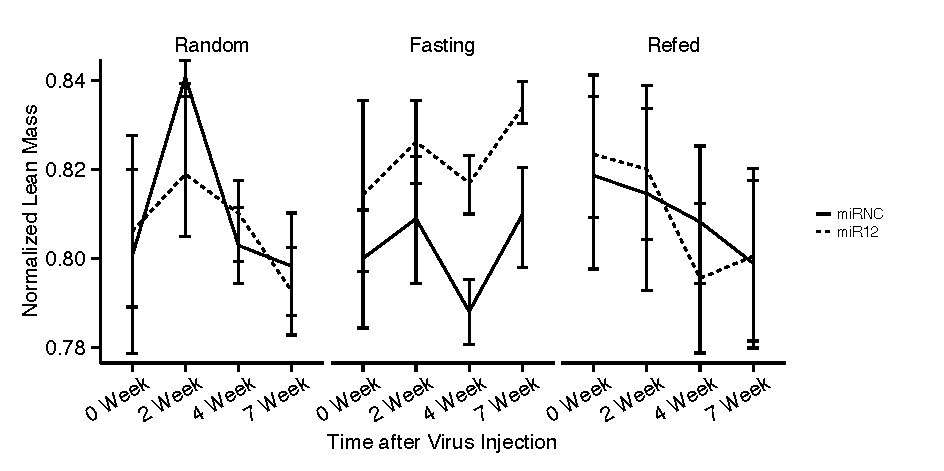
\includegraphics[width=1\textwidth]{figs/fig2-24 echoMRI lean.pdf}
%\caption[Body lean mass profile after PPP2R5C KD]{\footnotesize Body lean mass profile has no change after PPP2R5C knockdown. Mice were the same as Figure~\ref{fig:fig2.21}. Whole body lean mass composition was calculated from lean mass content normalized to body weight at each time point. Week 0 indicated fat composition before virus injection. n=5 or 6}
%\label{fig:fig2.24}
%\end{figure}

\begin{figure}[htbp]
\centering
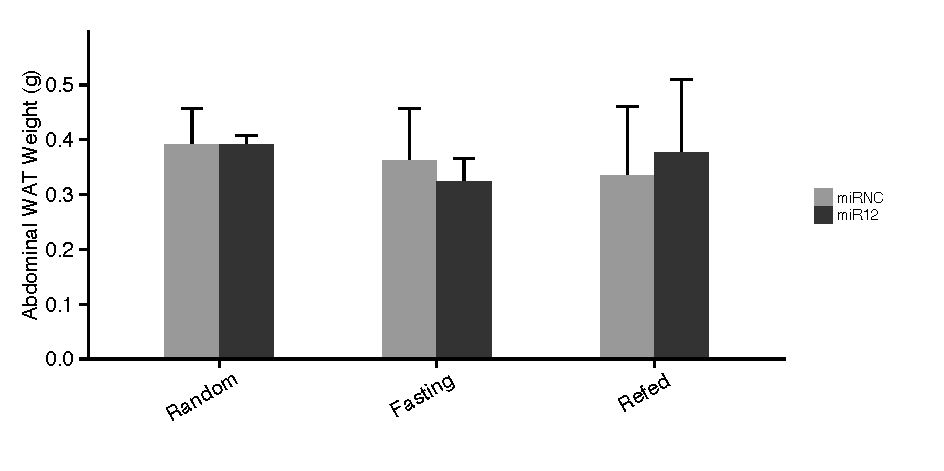
\includegraphics[width=1\textwidth]{figs/fig2-25 abd wat weight.pdf}
\caption[Abdominal fat after PPP2R5C KD]{\footnotesize Abdominal white adipose tissue (Abd.WAT) has no change after PPP2R5C knockdown. Mice were the same as Figure~\ref{fig:fig2.21}. After mice were treated with different nutritional statuses (Random, Fasting and Refed), Abd.WAT tissue was collected from each mouse and weighted before stored in -80\celsius{}. n=5 or 6.}
\label{fig:fig2.25}
\end{figure}

\subsection{PPP2R5C KD promotes glucose uptake \textit{in vivo} with better insulin sensitivity}

Since the liver is important for maintaining euglycemia, especially in the postprandial phase \cite{moore_regulation_2012}, I measured the blood glucose level for \textit{ad libitum} feeding ("Random"), 16 hour fasting ("Fasting"), and 16 hour fasting followed by 6 hour refeeding ("Refed") in control and knockdown mice (Figure~\ref{fig:fig2.26}). Surprisingly, there are no significant decreases in all three conditions, even given that PPP2R5C KD in cultivated hepatocytes increased glucose uptake (Figure~\ref{fig:fig2.15}). 

Although there is no change in blood glucose level after \gls{ppp2r5c} knockdown, the serum insulin concentration drops almost 2-fold after PPP2R5C knockdown (Figure~\ref{fig:fig2.28}) when mice are fed \textit{ad libitum}. In Fasting and Refed group, serum insulin levels are also decreased comparing with control mice. The decreased circulating insulin levels indicated the increased insulin sensitivity. Indeed, the insulin sensitivity index \cite{wallace_use_2004} in random and refed group are also increased in PPP2R5C knockdown mice (Figure~\ref{fig:fig2.29}). 

\begin{figure}[htbp]
\centering
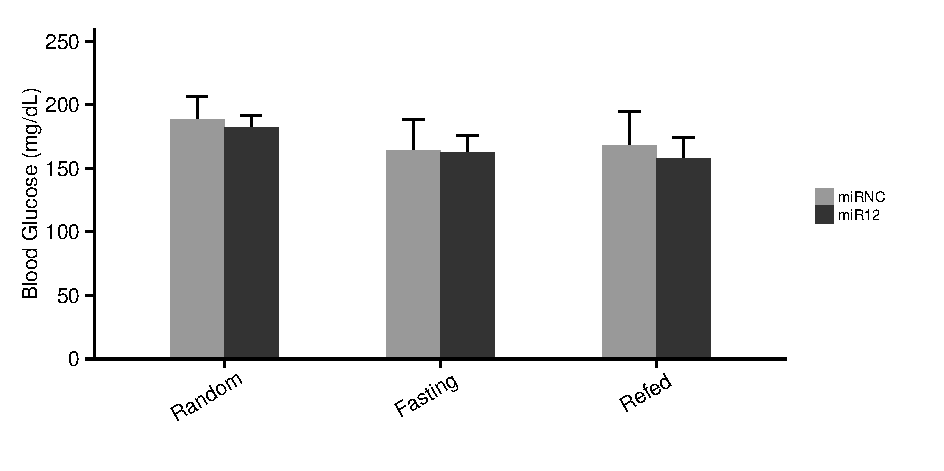
\includegraphics[width=1\textwidth]{figs/fig2-26 blood glucose.pdf}
\caption[Blood glucose after PPP2R5C KD]{\footnotesize Blood glucose level has no change after PPP2R5C knockdown. Mice were the same as Figure~\ref{fig:fig2.21}. Blood glucose level was immediately measured after sacrifice. n=5 or 6.}
\label{fig:fig2.26}
\end{figure}

\begin{figure}[htbp]
\centering
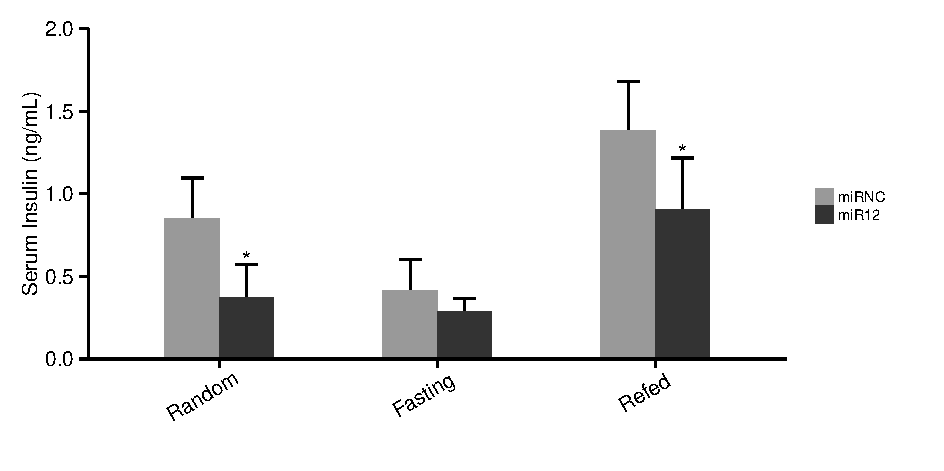
\includegraphics[width=1\textwidth]{figs/fig2-28 serum insulin.pdf}
\caption[Serum insulin drops after PPP2R5C KD]{\footnotesize Serum insulin drops after PPP2R5C knockdown in \textit{ad libitum} fed (Random) or 6-hour Refeeding after 16-hour fasting. Serum insulin was measured using ELISA kit for mouse insulin, and standard curve for ELISA was fitted from serial diluted insulin standards (0.1-6.9 ng/mL) with 5-parameter logistic model in R. * for p-value<0.05 by t-test in R for comparing miR12 to miRNC for each nutrition group. n=5 or 6.}
\label{fig:fig2.28}
\end{figure}


\begin{figure}[htbp]
\centering
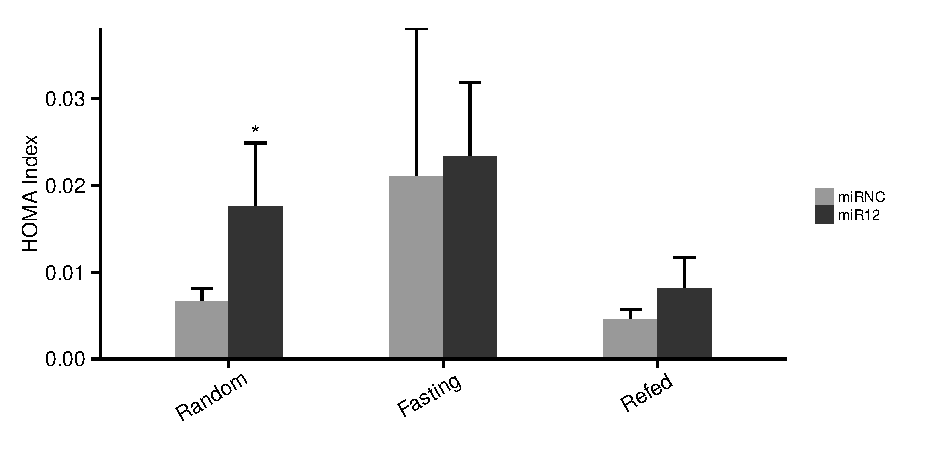
\includegraphics[width=1\textwidth]{figs/fig2-29 homa index.pdf}
\caption[ISI index increases after PPP2R5C KD]{\footnotesize Insulin sensitivity index (ISI) increases after PPP2R5C knockdown in \textit{ad libitum} fed (Random) or 6-hour re-feeding after 16-hour fasting. ISI index was calculated from the inverse of the product between blood glucose concentration and insulin concentration. * for p-value<0.05 by t-test in R for comparing miR12 to miRNC for each nutrition group. n=5 or 6}
\label{fig:fig2.29}
\end{figure}

Besides the increased insulin sensitivity, glucose uptake capacity is also increased in 6 hour fasted mice after \gls{ppp2r5c} knockdown, which is shown by the improved glucose tolerance in glucose tolerance test (GTT) (Figure~\ref{fig:fig2.43}). This piece of data is nicely correlated with the increased glucose uptake and glycolysis in cellular models (Hepa 1-6 cells and mouse primary hepatocytes, \cref{fig:fig2.11,fig:fig2.14,fig:fig2.15}). AUC analysis for \gls{gtt} data also demonstrates the decreased AUC in PPP2R5C knockdown (Figure~\ref{fig:fig2.44}). Although the absolute serum insulin levels from the same mouse in GTT experiment could not be calculated due to their level are below the limit of detection, raw O.D. 450 is used to estimate relative serum insulin level (Figure~\ref{fig:fig2.45}). And the relative serum insulin levels in PPP2R5C knockdown mice are even lower than control mice, given that they still have quicker glucose clearance rate (Figure~\ref{fig:fig2.43}). In sum, these data indicate PPP2R5C liver-specific knockdown mice have both increased insulin sensitivity and glucose uptake. 

\begin{figure}[htbp]
\centering
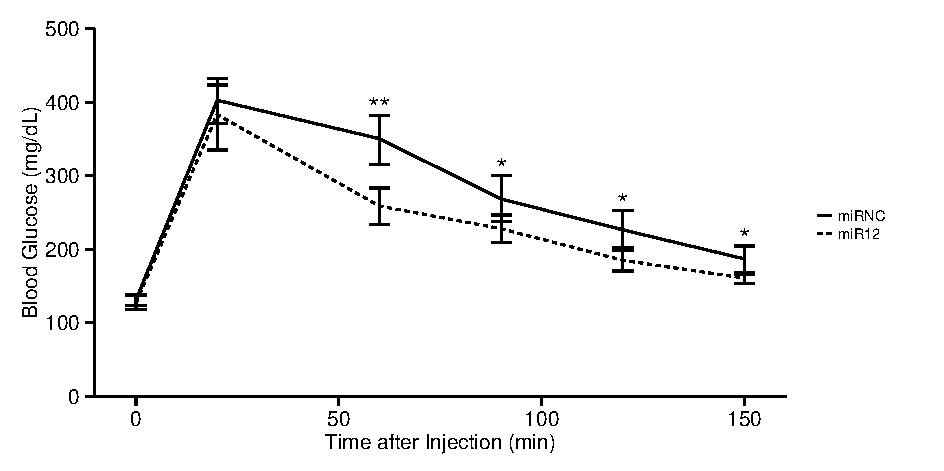
\includegraphics[width=1\textwidth]{figs/fig2-43 gtt.pdf}
\caption[GTT shows better glucose tolerance in PPP2R5C KD]{\footnotesize Glucose tolerance test (GTT) shows better glucose tolerance in PPP2R5C KD. GTT was performed 4 weeks after virus injection at dosage of 2g glucose/kg body weight. Glucose was solubilized in PBS and injected intraperitoneally. Blood glucose before injection was recorded as it for time 0 min, and also measured at time 20, 60, 90, 120 and 150 min. * and ** for p-value<0.05 and 0.01 by Wilcoxon signed-rank test in R for comparing miR12 to miRNC. n=12. Repeated Measures \gls{ANOVA} in R showed a significant difference in blood glucose changing profile with p-value of 0.0098.}
\label{fig:fig2.43}
\end{figure}

\begin{SCfigure}
\centering
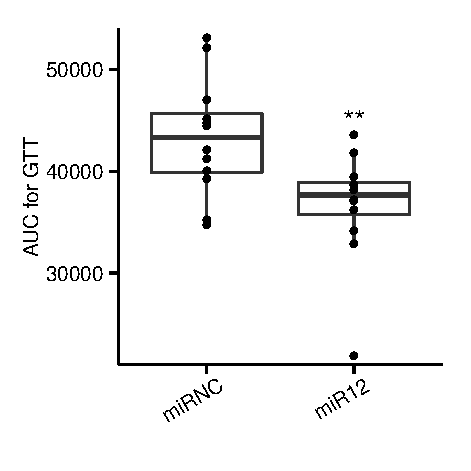
\includegraphics[width=0.5\textwidth]{figs/fig2-44 AUC for gtt.pdf}
\caption[AUC analysis for GTT results]{\footnotesize Area Under Curve (AUC) analysis for GTT blood glucose profile in Figure~\ref{fig:fig2.43}. ** for p-value<0.01 by t-test in R for comparing miR12 to miRNC. n=12.}
\label{fig:fig2.44}
\end{SCfigure}


\begin{figure}[htbp]
\centering
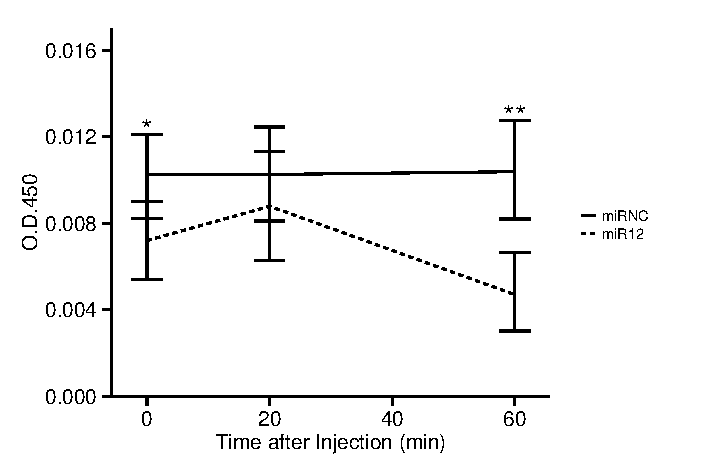
\includegraphics[width=1\textwidth]{figs/fig2-45 serum ins for gtt.pdf}
\caption[Serum insulin level in GTT]{\footnotesize Serum insulin relative level decreases in PPP2R5C. Due to O.D. 450 for some mice were even below the blank sample in the standard curve, absolute serum insulin level could not be calculated properly. Instead, raw O.D. 450 was employed to show the relative serum insulin level in GTT samples. * and ** for p-value<0.05 and 0.01 by two-sample t-test in R for comparing miR12 to miRNC. Repeated Measures \gls{ANOVA} in R showed a significant difference in serum insulin raw O.D. 450 profile with p-value of 0.0061. n=12.}
\label{fig:fig2.45}
\end{figure}


\subsection{PPP2R5C KD promotes anabolic changes in liver}

The increased glucose uptake in the liver after PPP2R5C KD indicates a more anabolic metabolism in hepatocytes in knockdown mice. In agreement with this, the liver has significant weight gain upon \gls{ppp2r5c} knockdown in all groups (Figure~\ref{fig:fig2.27}), instead of no systematic anabolic change in whole body weight or size of tissues beside the liver  (\cref{fig:fig2.22,fig:fig2.25}). The increase in Fasting and Refed group are even stronger than that in the Random group. In the postprandial phase, glucose is absorbed by hepatocytes to synthesize glycogen and lipids \cite{bechmann_interaction_2012,dashty_quick_2013}. The increase could be partially explained by the increase in liver glycogen (Figure~\ref{fig:fig2.30}) and triglyceride (Figure~\ref{fig:fig2.31}), even all these data are normalized to the liver weight. Without normalization, the increase in total liver triglyceride and glycogen would be even more.  Most strikingly, although glycogen levels drop in control livers upon fasting, as they enter a catabolic state to provide the rest of the organism with glucose, PPP2R5C knockdown livers displayed almost no drop in glycogen upon fasting (Figure~\ref{fig:fig2.30}).    

\begin{figure}[htbp]
\centering
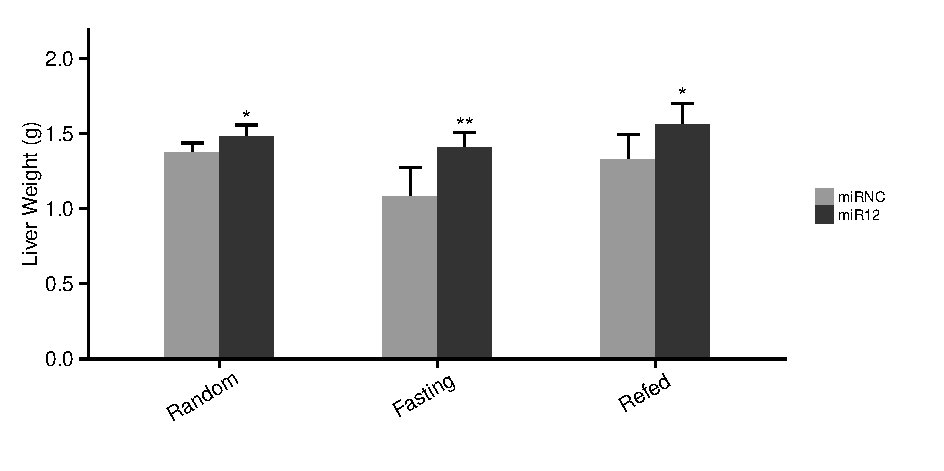
\includegraphics[width=1\textwidth]{figs/fig2-27 liver weight.pdf}
\caption[Liver weight increases after PPP2R5C KD]{\footnotesize Liver weight increases after PPP2R5C knockdown in all nutritional status. Mice were the same as in Figure~\ref{fig:fig2.21}. Dissected liver was weighted before aliquoting for cryosection, paraformaldehyde fixation and -80\celsius{} storage. n=5 or 6.}
\label{fig:fig2.27}
\end{figure}

\begin{figure}[htbp]
\centering
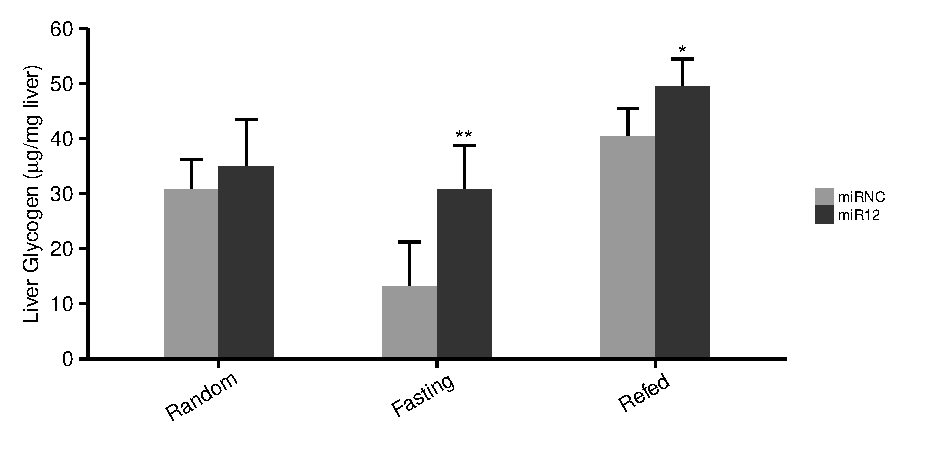
\includegraphics[width=1\textwidth]{figs/fig2-30 liver glycogen.pdf}
\caption[Liver glycogen increases after PPP2R5C KD]{\footnotesize Liver glycogen increases after PPP2R5C knockdown in fasting and refed. Mice were the same as in Figure~\ref{fig:fig2.21}. Frozen liver sample was pulverized in the tissue homogenizer with pre-cooling in liquid nitrogen. Glycogen was extracted from \textasciitilde150 mg liver powder and measured for glucose level after overnight amyloglucosidase digestion. * and ** for p-value<0.05 and 0.01 by t-test in R for comparing miR12 to miRNC for each nutrition group. n=5 or 6. }
\label{fig:fig2.30}
\end{figure}

Glucose is also used by hepatocytes for lipid biosynthesis. Combining data from \gls{gtt} experiment (Figure~\ref{fig:fig2.43}) and cell-autonomous increased glucose uptake lipogenesis in \textit{in vitro} cultivated hepatocytes (\cref{fig:fig2.15,fig:fig2.16}), implies the increased glucose uptake in the liver would also possibly shunted into lipid synthesis pathway. In agreement with this, mice with \gls{ppp2r5c} KD have significantly elevated triglyceride levels in their livers in the random feeding state. Due to two outliers of liver NEFA (Figure~\ref{fig:fig2.33}) in control mice in the random group, liver triglyceride levels in these two control mice are also higher, probably by passively increasing the re-esterification of NEFA into triglycerides in these two control mice. By \gls{ancova} (Analysis of Covariance) analysis with the liver NEFA as covariate, liver triglyceride in knockdown mice in the random group is found to be significantly higher (p-value=0.04). 

Although this lipid storage effect is visible after 7 week PPP2R5C knockdown (Figure~\ref{fig:fig2.31}), it is even more pronounced after 2 week knockdown (Figure~\ref{fig:fig2.57}), possibly due to the reduced knockdown efficiency upon counter-regulation over time, or compensatory regulatory mechanism developed over time. However, Oil Red O staining on the liver sample does not show visible change in lipid droplet (data not shown), which indicates the increased triglyceride storage is mainly microvesicular lipid droplets which are not easily visible under microscope after Oil Red O staining. 

\begin{figure}[htbp]
\centering
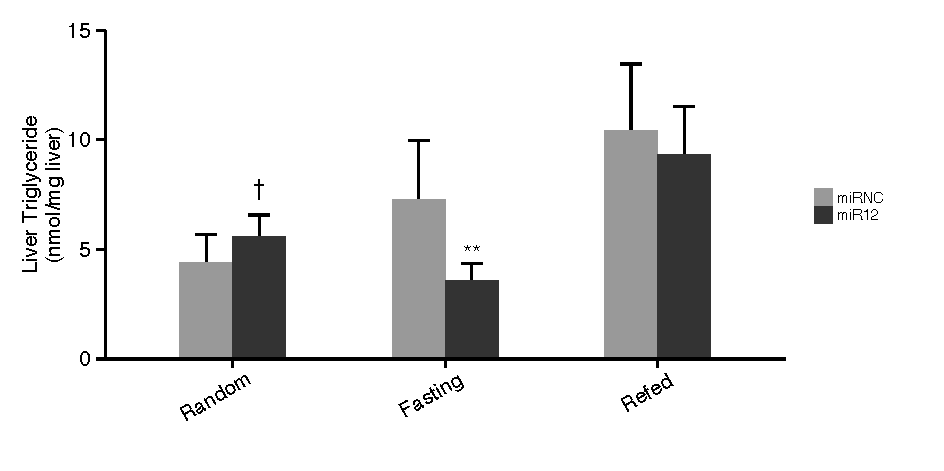
\includegraphics[width=1\textwidth]{figs/fig2-31 liver tag.pdf}
\caption[Liver triglyceride changes after PPP2R5C KD]{\footnotesize Liver triglyceride increases after PPP2R5C knockdown in random but decreases in fasting. Mice were the same as in Figure~\ref{fig:fig2.30}. Lipid fraction was extracted from liver by methanol-chloroform and triglyceride was measured as free glycerol released from lipase digestion. $\dagger$ for p-value<0.05 for \gls{ancova} analysis for comparing liver triglyceride between miRNC and miR12 in random fed, in which liver non-esterified fatty acids (\gls{nefa}) (Figure~\ref{fig:fig2.33}) as co-variate. ** for p-value<0.01 by t-test in R. n=5 or 6.}
\label{fig:fig2.31}
\end{figure}

\begin{figure}[htbp]
\centering
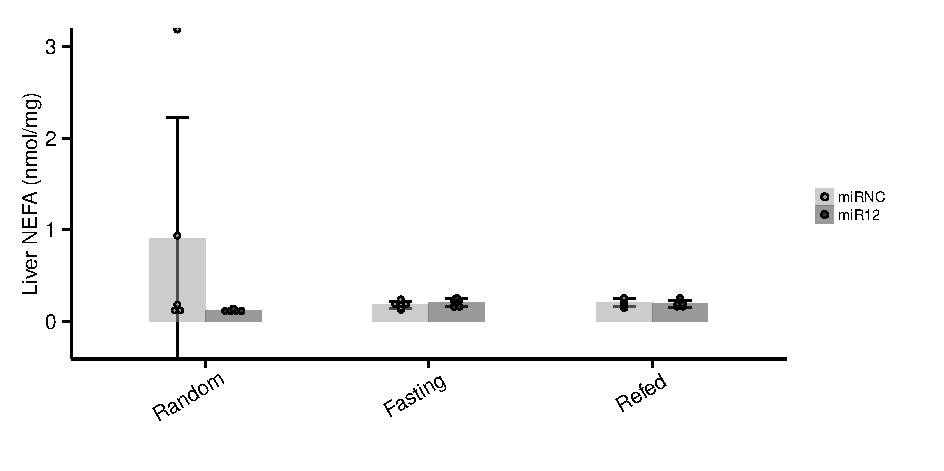
\includegraphics[width=1\textwidth]{figs/fig2-33 liver NEFA.pdf}
\caption[Liver NEFA has no change after PPP2R5C KD]{\footnotesize Liver NEFA level has no significant change after PPP2R5C knockdown in all feeding regimes. Mice were the same as in Figure~\ref{fig:fig2.30}. Lipid fraction was extracted from liver by methanol-chloroform and NEFA was measured. n=5 or 6.}
\label{fig:fig2.33}
\end{figure}

\begin{SCfigure}
\centering
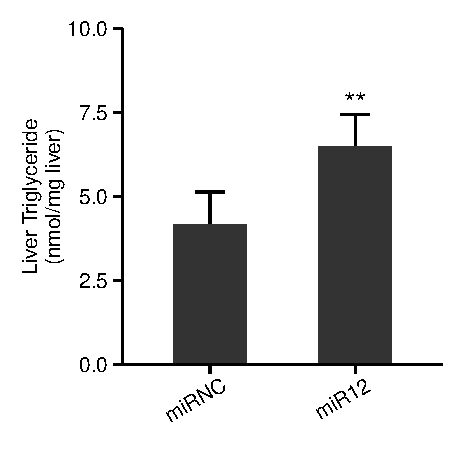
\includegraphics[width=0.5\textwidth]{figs/fig2-57 liver pilot tag.pdf}
\caption[Liver triglyceride increases in the pilot experiment]{\footnotesize Liver triglyceride increases after PPP2R5C knockdown in random fed. 8-10 week CL57BL/6 male mice were injected with adeno-associated virus packaged miRNA against mouse PPP2R5C (miR12) or scramble miRNA (miRNC) at 0.5 or 1$\times$10\textsuperscript{11} viral particles/mouse via tail injection in 100 $\mu$L PBS. And Injected mice was sacrificed after 2-week knockdown. For liver triglyceride analysis, data from low and high dose virus injection were combined. ** for p-value<0.01 by t-test in R for comparing miR12 to miRNC. n=5.}
\label{fig:fig2.57}
\end{SCfigure}


One possible explanation for the increased liver triglyceride levels could be the reduced liver fatty acid \textbeta{}-oxidation. However, the serum ketone body concentration of total ketone body species and hydroxybutyrate are maintained at the same level after \gls{ppp2r5c} KD (\cref{fig:fig2.37,fig:fig2.38}) at various feeding conditions. Total ketone body concentration are increased in the fasting group and decreased after refeeding for both control and PPP2R5C mice, which is expected since starvation in mice would increase \textbeta{}-oxidation activity in the liver and the following ketone body concentration in the circulation. Additionally, the hydroxybutyrate concentration normalized to total ketone body also did not show any relative change upon PPP2R5C KD (Figure~\ref{fig:fig2.39}). Circulating ketone body levels are not changed upon PPP2R5C KD is indicating that accumulation of hepatic triglyceride levels are not likely due to the impaired utilization in \textbeta{}-oxidation but presumably due to the increased \textit{de novo} lipogenesis, which have been demonstrated in \textit{in vitro} cell culture models (\cref{fig:fig2.16,fig:fig2.18}). 

\begin{figure}[htbp]
\centering
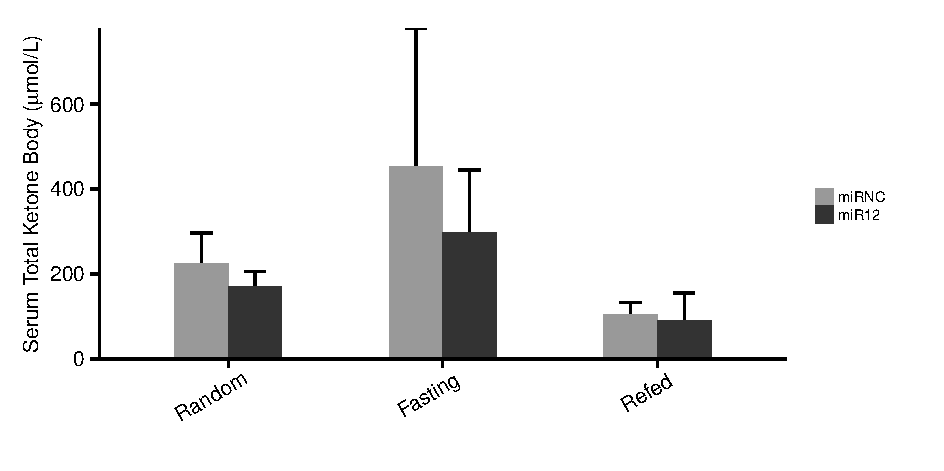
\includegraphics[width=1\textwidth]{figs/fig2-37 serum TKB.pdf}
\caption[Serum total ketone body upon PPP2R5C KD]{\footnotesize Serum total ketone body (TKB) does not change upon PPP2R5C knockdown in all feeding regimes. Mice were the same as in Figure~\ref{fig:fig2.30}. n=5 or 6.}
\label{fig:fig2.37}
\end{figure}

\begin{figure}[htbp]
\centering
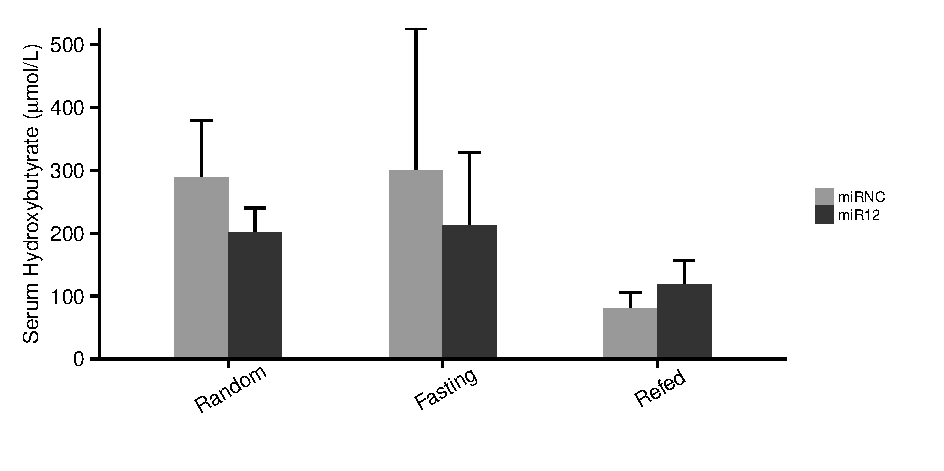
\includegraphics[width=1\textwidth]{figs/fig2-38 serum HB.pdf}
\caption[Serum hydroxybutyrate upon PPP2R5C KD]{\footnotesize Serum hydroxybutyrate (HB) concentration does not change upon PPP2R5C knockdown in all feeding regimes. Mice were the same as in Figure~\ref{fig:fig2.30}. n=5 or 6.}
\label{fig:fig2.38}
\end{figure}

\begin{figure}[htbp]
\centering
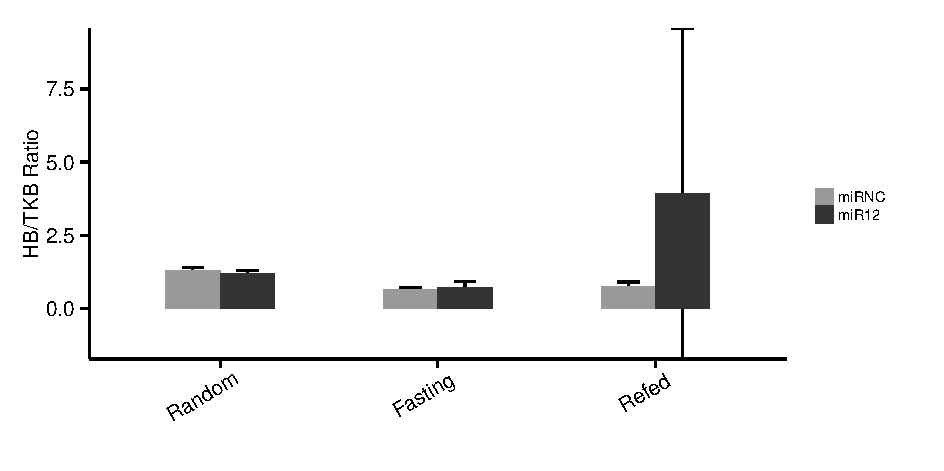
\includegraphics[width=1\textwidth]{figs/fig2-39 serum KB ratio.pdf}
\caption[Serum HB to TKB ratio upon PPP2R5C KD]{\footnotesize Serum HB to TKB ratio does not change upon PPP2R5C knockdown in all feeding regimes. Mice were the same as in Figure~\ref{fig:fig2.30}. n=5 or 6.}
\label{fig:fig2.39}
\end{figure}

Surprisingly, liver triglyceride levels drop significantly in PPP2R5C knockdown upon fasting (Figure~\ref{fig:fig2.31}). I have tested if this could be due to increased lipid secretion from the liver. Indeed, the serum triglyceride in fasting and refed group after PPP2R5C KD are increased significantly (Figure~\ref{fig:fig2.32}). This leads to a drop not only in triglyceride but also cholesterol in PPP2R5C knockdown livers upon fasting and refed (Figure~\ref{fig:fig2.35}). This raises the possibility of co-transportation of triglyceride and cholesterol out from the liver in the form of VLDL. Upon refeeding, PPP2R5C knockdown livers re-accumulated triglycerides very rapidly, reaching control levels within 6 hours of refeeding (Figure~\ref{fig:fig2.31}), consistent with elevated lipid biosynthesis rates in PPP2R5C knockdown livers. Taken together, PPP2R5C knockdown livers have more glucose uptake than control livers, thereby produce more triglycerides, and secrete elevated lipid amounts into circulation. The steady state levels of triglyceride in PPP2R5C knockdown livers likely reflect this balance between increased biosynthesis and increased secretion, leading to a drop in the liver triglyceride upon fasting when less dietary glucose is available for lipid biosynthesis. If the serum triglyceride and liver triglyceride are considered together, the overall triglyceride at least in random and refed condition are increased in knockdown mice.

\begin{figure}[htbp]
\centering
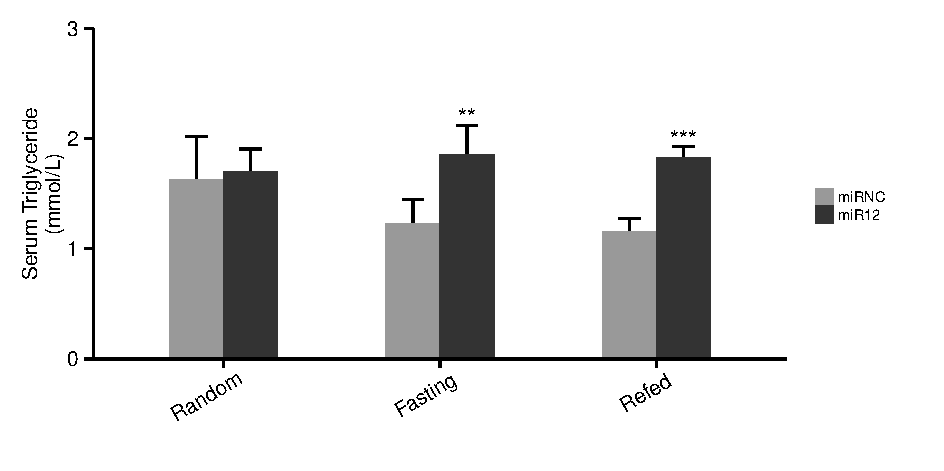
\includegraphics[width=1\textwidth]{figs/fig2-32 serum tag.pdf}
\caption[Serum triglyceride changes after PPP2R5C KD]{\footnotesize Serum triglyceride increases after PPP2R5C knockdown in fasting and refed. Mice were the same as in Figure~\ref{fig:fig2.30}. 2 $\mu$L serum from these mice was measured as free glycerol released from lipase digestion. ** and *** for p-value<0.01 and 0.001 by t-test in R. n=5 or 6.}
\label{fig:fig2.32}
\end{figure}

Lipoactive hormones such as epinephrine, norepinephrine, glucagon, thyrotropin, and adrenocorticotropin release free fatty acids (Serum \gls{nefa}) into serum from lipolysis in adipose tissues. And the liver can re-absorb almost 75\% of the serum NEFA to re-esterify them into triglyceride and release into serum as VLDL particle. Upon \gls{ppp2r5c} knockdown, the steady state level of serum NEFA in random and fasting feeding regime are not changed (Figure~\ref{fig:fig2.34}), which further indicates the increased lipid storage is rather sourced from \textit{de novo} lipogenesis in the liver. In refeeding, mice with PPP2R5C knockdown even have significant increased serum NEFA. During refeeding, serum NEFA could also be originated from the food intake. And it is possible the liver lipid synthesis capacity has already reached its plateau and the NEFA is accumulated in the serum to have a higher concentration in PPP2R5C knockdown mice than the control. This postulation also fits with the fact that the liver triglyceride in refed condition stays at very high level but there is still more triglyceride released into serum, which suggests higher triglyceride synthesis and secretion in the liver during refed.

\begin{figure}[htbp]
\centering
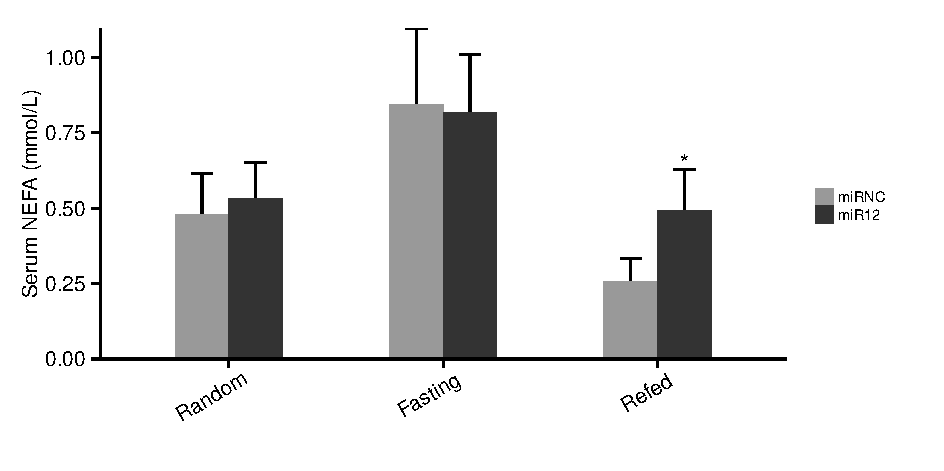
\includegraphics[width=1\textwidth]{figs/fig2-34 serum NEFA.pdf}
\caption[Serum NEFA changes in refed]{\footnotesize Serum NEFA is decreased in refed. Mice were the same as in Figure~\ref{fig:fig2.30}. Lipid fraction was extracted from liver by methanol-chloroform and triglyceride was measured as free glycerol released from lipase digestion. 2 $\mu$L serum from these mice was measured for NEFA. * for p-value<0.05 by t-test in R. n=5 or 6.}
\label{fig:fig2.34}
\end{figure}


\section{PPP2R5C negatively regulates VLDL secretion in the liver}

Given the fact that serum triglyceride was increased during fasting and refed, I performed a more detailed analysis of serum lipid composition by \gls{fplc} (Fast Performance Liquid Chromatography) fractionation of serum, in order to find which lipoprotein particle was responsible for increased serum triglyceride. \gls{vldl}, \gls{idl}, \gls{ldl} and \gls{hdl} could be nicely separated on a high resolution size-exclusion chromatography column. In Random group, mice after \gls{ppp2r5c} KD has no difference in serum lipoprotein particle profile (Total protein content (A280) in lipoprotein fractions is shown in Figure~\ref{fig:fig2.42}). However, there is a significant increase in \gls{vldl} fraction (approximately 5-fold increase) in Fasting and Refed group after PPP2R5C knockdown. In Fasting group, even there is a slight increase in HDL intensity, the relative VLDL intensity normalized to HDL is still increasing dramatically in knockdown mice. 

\begin{figure}[htbp]
\centering
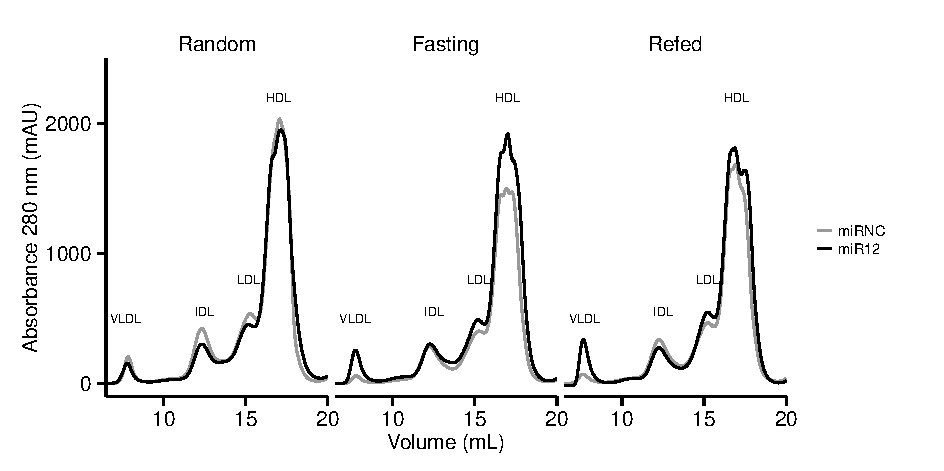
\includegraphics[width=1\textwidth]{figs/fig2-42 fplc_profile.pdf}
\caption[Serum FPLC profile]{\footnotesize Increased VLDL fraction after PPP2R5C KD. Serum lipoprotein particles were analyzed by FPLC. 200 $\mu$L pooled serum from 5 or 6 mice in the same virus and feeding group was subjected to FPLC separation on high-resolution size-exclusion chromatography. FPLC profile was recorded as UV 280nm, which was the indicator for protein concentration. Separated serum was collected in fractions of 0.5 mL. Mice were the same as in Figure~\ref{fig:fig2.30}.}
\label{fig:fig2.42}
\end{figure}

Concordantly, triglyceride distribution profile in serum is also agreed with increased VLDL intensity (Figure~\ref{fig:fig2.40}). Although triglyceride concentrations in knockdown mice from Refed group have higher background level, the background subtracted intensity of VLDL triglyceride peak is distinctly higher than that for control mice in the same feeding group. Quantification of VLDL peak apex and peak area both in FPLC and triglyceride profile is shown in Figure~\ref{fig:fig2.58}. VLDL particles are lipoprotein particles synthesized in the liver and secreted into the blood stream for transporting endogenous triglyceride, cholesterol, phospholipids and cholesterol esters \cite{gibbons_synthesis_2004}. Comparing with other lipoprotein particles, VLDL has the highest percentage of triglyceride, and could explain the significant increase in serum triglyceride in the form of VLDL. The increased VLDL secretion is also observed in human upon increased hepatic \textit{de novo} lipogenesis \cite{schwarz_hepatic_2003}. 


\begin{figure}[htbp]
\centering
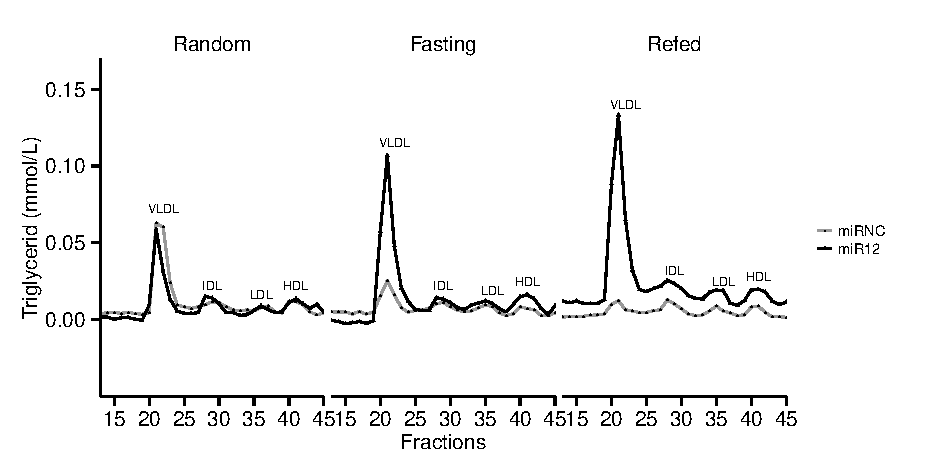
\includegraphics[width=1\textwidth]{figs/fig2-40 fplc_tag.pdf}
\caption[Triglyceride concentration in lipoprotein particles]{\footnotesize Triglyceride concentration profile correlated with its FPLC profile. 160 $\mu$L from each fraction was used to measure triglyceride concentration as free glycerol released from lipase digestion.}
\label{fig:fig2.40}
\end{figure}

\begin{figure}[htbp]
\centering
\includegraphics[width=1\textwidth]{figs/fig2-58 vldl_peak.pdf}
\caption[VLDL peak analysis]{\footnotesize Quantification of VLDL peak apex and area. Start and end point for each peak in Figure~\ref{fig:fig2.42} were manually selected by examining the emerging and vanishing time point for each peak comparing with the background. Peak Apex and Area were calculated in R by finding maximal intensity and trapezoid integration from start point to end point for VLDL peak.}
\label{fig:fig2.58}
\end{figure}

In agreement with the increased serum VLDL fraction, cholesterol level in this fraction has also increased (Figure~\ref{fig:fig2.41}), although contributes a small share in total serum cholesterol. The biggest cholesterol peak is from HDL, which is known to carry a high percentage of cholesterol. And this minor contribution from VLDL cholesterol also explain why there is no significant gain in the serum cholesterol level given the increased cholesterol secretion from the liver (Figure~\ref{fig:fig2.35}). Liver cholesterol is probably passively packaged into the VLDL particle together with the triglyceride and released into the serum, due to the increased lipogenesis in the liver upon PPP2R5C KD. However, the total serum cholesterol levels have not change (Figure~\ref{fig:fig2.36}) since the cholesterol from VLDL is only a minor fraction comparing to the cholesterol from IDL and HDL peaks (Figure~\ref{fig:fig2.41}), which are not changed dramatically upon PPP2R5C KD (Figure~\ref{fig:fig2.42}). This data further validates the hypothesis that increased glucose uptake in the liver is shunted into lipogenesis and eventually released into the serum in the form of \gls{vldl} after \gls{ppp2r5c} knockdown. 


\begin{figure}[htbp]
\centering
\includegraphics[width=1\textwidth]{figs/fig2-41 fplc_chol.pdf}
\caption[Cholesterol concentration in lipoprotein particles]{\footnotesize Cholesterol concentration profile in various lipoprotein particles. 40 $\mu$L from each fraction was used to measure cholesterol concentration.}
\label{fig:fig2.41}
\end{figure}


\begin{figure}[htbp]
\centering
\includegraphics[width=1\textwidth]{figs/fig2-35 liver chol.pdf}
\caption[Liver cholesterol drops upon PPP2R5C KD]{\footnotesize Liver cholesterol is dropped in fasting and refed after PPP2R5C KD. Mice were the same as in Figure~\ref{fig:fig2.30}. Lipid fraction was extracted from liver by methanol-chloroform and cholesterol was directly measured. * and ** for p-value<0.05 and 0.01 by t-test in R for comparing miR12 to miRNC for each nutrition group. n=5 or 6.}
\label{fig:fig2.35}
\end{figure}

\begin{figure}[htbp]
\centering
\includegraphics[width=1\textwidth]{figs/fig2-36 serum chol.pdf}
\caption[Serum cholesterol level remains no change]{\footnotesize Serum cholesterol has no change after PPP2R5C KD in all feeding regimes. Mice were the same as in Figure~\ref{fig:fig2.30}. 2 $\mu$L serum was used to measure cholesterol directly. n=5 or 6.}
\label{fig:fig2.36}
\end{figure}

In summary, due to the increased lipogenesis derived from the increased glucose uptake in the liver after PPP2R5C KD, VLDL secretion from the liver is also increased and contributing to the anabolic storage of glucose in the liver. The increased glucose clearance capacity of the liver after PPP2R5C KD enable the efficient euglycemic control with less insulin secretion from the pancreas in the postprandial phase or massive oral or enteral glucose load (like GTT). The increased glucose absorbed by the liver is  directed either to glycogen synthesis or lipid storage and secretion. It is known that the hepatic glycogen deposition is partially driven by the increased liver glucose uptake, metabolite or hormonal signaling from port vein, and partly by gluconeogenesis pathway \cite{radziuk_hepatic_2001}. In PPP2R5C knockdown mice, the increased glucose uptake will probably also explain the increased liver glycogen phenotype. Another possible anabolic change after increased glucose uptake is storing glucose as triglyceride through \textit{de novo} lipogenesis. The increased glucose flux to the liver after PPP2R5C KD could potentially activate lipogenic gene expression via multiple pathways. Glucose is considered as signaling metabolite for activating glycolytic and lipogenic pathways \cite{foufelle_new_2002}. In following sections, I will have more data to show the direct and indirect link from PPP2R5C to glucose metabolism.


\section{PPP2R5C's substrates in metabolism control}

\subsection{PPP2R5C's substrates include multiple metabolic regulators}

\gls{ppp2r5c} is a regulatory subunit of \gls{PP2A}, thought to provide substrate specificity to the phosphatase holoenzyme. However, given the phenotype I have observed from \textit{in vitro} and \textit{in vivo} knockdown of PPP2R5C, it is not possible to make a direct link from PP2A to the negative regulation of glycolysis and lipogenesis. There must be some intermediate molecular links from PP2A to the regulation of glycolysis and lipogenesis, such as glycolytic and lipogenic gene activation by some transcription factors and kinases. A reasonable educational guess is that PPP2R5C regulates glycolytic and lipogenic gene activation through de-phosphorylating metabolic regulators. 

Therefore, I performed a proteomic approach to identify target substrates that bind PPP2R5C. And potential substrates involved in metabolism control would provide a clue to elucidate the mechanism of PPP2R5C's negative regulation in glycolysis and lipogenesis. However, phosphatase substrate discovery is difficult. Beside occasionally successes in finding phosphatase interacting substrates, there are few reports regarding system-wide substrate identification for phosphatases, mostly protein tyrosine phosphatases \cite{boubekeur_new_2011,flint_development_1997,wu_identification_2006}. In the  case for protein tyrosine phosphatases, a substrate trapping mutant competes with its endogenous counterpart for substrates. Due to its structural simplicity (single subunit and verified catalytic dead mutant, usually a cysteine to serine mutation in catalytic active center), protein tyrosine phosphatase is much easier for pulling down its binding substrates. For Serine/Threonine kinases, MAP kinase phosphatase-1 is another success example of substrate trapping \cite{kinney_histone_2009}.

Protein-protein interactions between phosphatases and substrates are notoriously transient and difficult to detect via conventional methods, such as co-immunoprecipitation and pull-down strategies. I have tested these conventional methods and abandoned them for PPP2R5C substrate isolation due to the high background and no detectable new band on SDS-PAGE gel. Here in the thesis project, I employed the BioID method \cite{roux_promiscuous_2012}   to identify PPP2R5C interacting proteins, including its potential substrates. A fusion between PPP2R5C and the biotin ligase \gls{bira} mutant (BirA*) was expressed in Hepa 1-6 cells. The mutant biotin ligase (R118G) has been shown to be able to generate reactive biotin (biotin-5'-AMP) and ligate biotin onto proteins \textit{in vitro} \cite{choi-rhee_promiscuous_2004,cronan_targeted_2005}. With the co-expression of substrate trapping mutant of PP2A catalytic subunit C, fusion protein from PPP2R5C and BirA* led to \textit{in vivo} biotinylation of PPP2R5C interacting proteins, which can subsequently be isolated by collecting cellular lysates and streptavidin pulldown (Figure~\ref{fig:fig2.46}). 

By this way, these potential substrates with weak interactions with PPP2R5C would have a higher chance to be identified by the Western blot or mass spectrometry with very low background since it is possible to apply very stringent washing steps. BirA* was fused to either the N-terminus or the C-terminus of PPP2R5C (Myc-BirA-PPP2R5C and PPP2R5C-BirA-HA respectively), and Myc or HA-tagged BirA* alone was used as a negative control. In addition, the catalytic dead mutation (D85N), which was known to eliminate the phosphatase activity \cite{ogris_catalytically_1999} by disrupting the Mg\textsuperscript{2+} binding in the active center, was introduced into the catalytic subunit of \gls{PP2A} (PP2CA). This design was the first successful attempt to perform a substrate trapping assay for PP2A, and expected to employ \gls{PP2A}'s substrate-trapping mutation might extend the duration of interaction between \gls{PP2A} and its substrate proteins. Then there will be more \textit{in vivo} biotinylation on these substrates when the PP2A catalytic dead mutant is co-expressed. 

\begin{figure}[htbp]
\centering
\includegraphics[width=1\textwidth]{figs/fig2-46 bioID scheme.png}
\caption[PPP2R5C substrate trapping scheme]{\footnotesize PPP2R5C containing PP2A holoenzyme substrate trapping and \textit{in vivo} biotinylation of its substrates.}
\label{fig:fig2.46}
\end{figure}

In the BioID experiment, various known regulators of the liver metabolism were found to be interacting with \gls{ppp2r5c}, including \gls{AMPK} \textbeta{}1, \gls{HIF1a}, \gls{s6k}, \gls{stat3} (Figure~\ref{fig:fig2.47a}). Comparing to either Myc-\gls{bira}* or BirA*-HA controls, HIF1\textalpha{} has increased biotinylation, which is shown as stronger band after streptavidin pulldown and detection with total antibodies for individuals. When co-expressed with the substrate trapping mutant of \gls{PP2A} catalytic subunit, the interaction between PPP2R5C and its substrates is further increased. This proves the success of the substrate trapping mutant of PP2A, which could potentially increase the binding duration of substrates to PPP2R5C containing PP2A holoenzyme. For \gls{s6k} and \gls{stat3}, similar results are also observed and indicating their possibility of being PPP2R5C's substrates. With \gls{AMPK}'s various subunits tested in substrate trapping, including \textalpha{}, \textbeta{}1 and \textbeta{}2, only \textbeta{}1 subunit has been found to be a potential PP2A substrate. In contrast, no binding of PPP2R5C to SREBP-1, or a panel of negative control proteins are detected, including HSP90, YAP, TSC1 and RpL26 (Figure~\ref{fig:fig2.47b}).

\begin{figure}[!t]
\centering
	\begin{subfigure}[t]{0.48\textwidth}
	\subcaption{Western blot of PPP2R5C substrate}
	\includegraphics[width=1\textwidth]{figs/fig2-47 bioid target1.pdf}
    \label{fig:fig2.47a}
	\end{subfigure} %
~
	\begin{subfigure}[t]{0.48\textwidth}
	\subcaption{Negative controls of PPP2R5C substrate trapping}
	\includegraphics[width=1\textwidth]{figs/fig2-48 bioid target2.pdf}
    \label{fig:fig2.47b}
	\end{subfigure}
\caption[Metabolic regulators as PPP2R5C's substrates]{\footnotesize PPP2R5C's substrates involved in metabolic control. (a) PPP2R5C interacting proteins were validated by western blot. SREBP-1, Tubulin or Actin were used as non-interacting controls. (b) AMPK \textbeta{}1 subunit and several other negative controls were used to validate the specificity of PPP2R5C's substrate trapping in an independent repeat experiment.}
\label{fig:fig2.47}
\end{figure}


\subsection{AMPK is PPP2R5C's substrate involved in glucose uptake}

The \gls{AMPK} is a master regulator in energy homeostasis. It is a trimeric heterogenous complex composed of \textalpha{} for catalytic activity, \textbeta{} for regulatory function, and \textgamma{} for sensing AMP/\gls{ATP} ratio. Given the interaction between \gls{AMPK} \textbeta{}1 and \gls{ppp2r5c} (Figure~\ref{fig:fig2.47}), there might also be some functional link between \gls{PP2A} and \gls{AMPK}. Indeed, there were several reports showed the \gls{AMPK} phosphorylation is negatively regulated by \gls{PP2A} \cite{park_ampk_2013,wang_pp2a_2010,wu_activation_2007}. However, which regulatory subunit in \gls{PP2A} is responsible for \gls{AMPK} de-phosphorylation is still unknown. With PPP2R5C knockdown, the PPP2R5C containing sub-pool of \gls{PP2A} holoenzyme is reduced. \gls{AMPK} activity is markedly increased upon PPP2R5C knockdown with different methods, either the adenovirus mediated knockdown (Figure~\ref{fig:fig2.50a}) or an inducible shRNA stable cell line (Figure~\ref{fig:fig2.50b}). This data clearly shows that PPP2R5C is at least one of the regulatory subunit of \gls{PP2A} involved in \gls{AMPK} inhibition in liver originated cell lines. Accordingly, \gls{AMPK} activity change was further validated by the changes in its downstream effectors' activity such as ACC1 phosphorylation, TBC1D1 phosphorylation. For ACC1 phosphorylation, it has been well characterized as AMPK target and mediating AMPK's inhibition on lipogenesis \cite{ha_critical_1994,sullivan_inhibition_1994}. It is known that TBC1D1, the mouse homolog for human AS160, is an upstream regulator for Glut1 translocation and  phosphorylation at S700 of TBC1D1 promotes glucose uptake \cite{vichaiwong_contraction_2010,zhou_akt_2008}. This raises the possibility of AMPK activation after PPP2R5C knockdown is mediating the increased glucose uptake phenotype (\cref{fig:fig2.14,fig:fig2.15}).

\begin{figure}[htbp]
\centering
	\begin{subfigure}[t]{0.48\textwidth}
	\subcaption{AMPK activity increases upon PPP2R5C KD}
	\includegraphics[width=1\textwidth]{figs/fig2-50a ampk increase AV shR3.pdf}
    \label{fig:fig2.50a}
	\end{subfigure} %
~
	\begin{subfigure}[t]{0.48\textwidth}
	\subcaption{Activity increase of AMPK and its down-steam effectors}
	\includegraphics[width=1\textwidth]{figs/fig2-50b ampk increase.pdf}
    \label{fig:fig2.50b}
	\end{subfigure}
\caption[AMPK activity increases upon PPP2R5C knockdown]{\footnotesize AMPK activity is up-regulated upon PPP2R5C knockdown. (a) AMPK activity is increased after PPP2R5C knockdown by adenovirus packaged shR3 comparing to shRNC (PPP2R5C KD vs Control KD). (b) Inducible shR3 and shR6 (PPP2R5C KD1 and KD2) were used to examine the AMPK activity change in order to eliminate any virus-mediated effect in (a).}
\label{fig:fig2.50}
\end{figure}

\subsection{HIF1\texorpdfstring{\textalpha}{a}{} is PPP2R5C's substrate involved in glycolysis and lipogenesis}

The \gls{HIF1a} is also known for controling glycolysis and lipogenesis in the liver \cite{ochiai_disruption_2011,nath_hepatocyte-specific_2011,li_altered_2006,li_intermittent_2005, wang_ablation_2009}. The interaction between HIF1\textalpha{} and PPP2R5C, which is demonstrated by the substrate trapping in Figure~\ref{fig:fig2.47}, indicates that HIF1\textalpha{} could also be one of PPP2R5C's potential substrates involved in metabolism control. However, there is no phospho-specific antibody commercially available for HIF1\textalpha{}. Then I used Phos-tag\textsuperscript{\textregistered} gel to evaluate the functional relevance of PPP2R5C knockdown on HIF1\textalpha{}'s phosphorylation status (Figure~\ref{fig:fig2.51}). Phos-tag\textsuperscript{\textregistered} gel is made from an acrylamide analog containing chemical group for binding phosphorylated ions specifically \cite{tomida_detection_2008,kinoshita_improved_2011,marelli-berg_molecular_2012,hosokawa_quantitative_2010,kinoshita_separation_2009}. When protein is phosphorylated, its mobility in Phos-tag\textsuperscript{\textregistered} gel will be retarded. As a result, phosphorylated and non-phosphorylated proteins will be separated and protein phosphorylation with unknown site could be possibly examined without phospho-specific antibodies. The HIF1\textalpha{} has increased phosphorylated form upon PPP2R5C knockdown, and this phosphorylation is also validated by CIP treatment (Figure~\ref{fig:fig2.51}). These data suggest the PPP2R5C knockdown increases the phosphorylation of HIF1\textalpha{}.

\begin{figure}[htbp]
\centering
\includegraphics[width=0.9\textwidth]{figs/fig2-51 hif phospho.pdf}
\caption[HIF1\textalpha's phosphorylation analysis by Phos-tag\textsuperscript{\textregistered}]{\footnotesize HIF1\textalpha{}'s phosphorylation is increased after PPP2R5C KD. HIF1\textalpha{}'s phosphorylation status was evaluated in Phos-tag\textsuperscript{\textregistered} gel after inducible shR3 and shR6 expression (PPP2R5C KD1 and KD2).}
\label{fig:fig2.51}
\end{figure}

In agreement with the phosphorylation increase upon \gls{ppp2r5c} knockdown, \gls{HIF1a}'s transcriptional activity is also up-regulated after PPP2R5C knockdown (Figure~\ref{fig:fig2.53}) in mouse primary hepatocytes. Four canonical down-stream targets of HIF1\textalpha{} are all increased in mRNA level. Three of these four targets are involved in glycolysis, including LDH\textalpha{}, HK2, and PKM2, could help to explain the increased glycolysis after PPP2R5C knockdown. In addition, the activation of HIF1\textalpha{} in the mouse liver by hypoxia has been shown to activate SREBP-1 consequently and promote lipid accumulation in the liver \cite{li_intermittent_2005}. Interaction between HIF1\textalpha{} and PPP2R5C provides a possible indirect link from PPP2R5C KD to lipogenic gene activation, and elucidates the strong lipid storage phenotype in mouse primary hepatocytes after PPP2R5C KD (Figure~\ref{fig:fig2.16}). The next missing link in this hypothesis would be the SREBP-1 activation.

\begin{figure}[!tbp]
\centering
\includegraphics[width=1\textwidth]{figs/fig2-53 hif target 1st hepa.pdf}
\caption[HIF1\textalpha's transcriptional activity increases upon PPP2R5C KD]{\footnotesize HIF1\textalpha{}'s transcriptional activity is increased after PPP2R5C KD. Four HIF1\textalpha{}'s targets were examined for its total mRNA level in mouse primary hepatocytes after PPP2R5C KD.}
\label{fig:fig2.53}
\end{figure}

\subsection{Microarray analysis of PPP2R5C KD in mouse liver}\label{sec:sec254}

In parallel with the substrate trapping experiment,  I also performed the microarray analysis on PPP2R5C knockdown cells and tissue samples to shed more light on the mechanism behind the increased glycolysis and lipogenesis phenotype. Mouse primary hepatocytes, Hepa 1-6 cells and mouse livers with or without PPP2R5C were submitted for microarray analysis. For mouse liver samples, different feeding groups was also included. Differentially expressed gene list was generated based on 2-fold change cutoff for all feeding conditions and cell culture with PPP2R5C knockdown by the limma package in R. 

In order to find relevant transcription factors (TF) involved in the metabolic change and further link these TFs to PPP2R5C substrates, I performed an enrichment analysis for activated or inhibited TFs after PPP2R5C KD in mouse tissues or cell models. TF enrichment analysis was done with an online web server of TFactS \cite{essaghir_transcription_2010}. The TFactS analysis is analyzing the differentially expressed genes with 2-fold cutoff and finding the most possible TFs for these genes based on published known target genes of various TFs. The Transcription factor (TF) enrichment analysis from differentially expressed genes in mouse liver with PPP2R5C KD has shown the increased SREBP-1 activity after PPP2R5C KD both in cell and tissue samples (\cref{tab:tab2.1,tab:tab2.2,tab:tab2.3,tab:tab2.4}).

During refeeding, both SREBP-1 and HIF1\textalpha{} were enriched based on their potential target gene activation (Table~\ref{tab:tab2.1}). The activated TF lists upon PPP2R5C KD in fasting and random fed are shown in Supplementary \cref{tab:tab2.2,tab:tab2.3}. The activated TF list upon PPP2R5C KD in mouse primary hepatocyte and Hepa 1-6 is shown in Supplementary Table~\ref{tab:tab2.4}. All these lists have SREBP-1 (gene name SREBF1) in the activation TF list based on target gene expression. HIF1\textalpha{}, although only significant in FDR controlled p-value, is also enriched in activated TF list. The activation of HIF1\textalpha{} and SREBP-1 further supports HIF1\textalpha{} as potential PPP2R5C's substrate, and mediating the increased lipogenesis phenotype after PPP2R5C KD, possibly through the downstream activation of SREBP-1. 

\begin{table}[htbp]
\begin{center}
\begin{threeparttable}
\caption{Activated TFs in mouse liver upon PPP2R5C KD during refed.}
\label{tab:tab2.1}
\begin{footnotesize}
\begin{tabular}{lcc}
\toprule
\multicolumn{1}{c}{Transcription Factor}&\multicolumn{1}{c}{P-value}&\multicolumn{1}{c}{FDR control (B-H)\tnote{a}.}\tabularnewline
\midrule
\textbf{SREBF1}&$0.00038$&$0.001613$\tabularnewline
TP53&$0.00266$&$0.003226$\tabularnewline
ID3&$0.00921$&$0.004839$\tabularnewline
ID2&$0.00921$&$0.006452$\tabularnewline
NOTCH2&$0.01226$&$0.008065$\tabularnewline
ID1&$0.01226$&$0.009677$\tabularnewline
PPARA&$0.03340$&$0.011290$\tabularnewline
SMAD1&$0.04233$&$0.012900$\tabularnewline
NR2F1&$0.04825$&$0.014520$\tabularnewline
\textbf{HIF1A}&$0.06579$&$0.016130$\tabularnewline
STAT1&$0.07446$&$0.017740$\tabularnewline
E2F1&$0.07917$&$0.019350$\tabularnewline
FOXO1&$0.08369$&$0.020970$\tabularnewline
CEBPA&$0.09721$&$0.022580$\tabularnewline
SREBF2&$0.10000$&$0.024190$\tabularnewline
\bottomrule
\end{tabular}
\end{footnotesize}
\begin{tablenotes}  
\item[a] \scriptsize{Adjusted p-value (false discovery rate) by Benjamini-Hochberg method  \cite{benjamini_controlling_1995}}.
\end{tablenotes}
\end{threeparttable}
\end{center}
\end{table}


\subsection{SREBP-1 is involved in lipogenesis phenotype}

In Section~\ref{sec:sec254}, SREBP-1 is found to be activated upon PPP2R5C knockdown. Since SREBP-1 is the master regulator in lipogenesis, and its over-expression in the liver cause fatty liver \cite{horton_srebps:_2002}. Although SREBP-1 was not interacting with \gls{ppp2r5c} in substrate trapping experiment, SREBP-1 could still be involved in the lipogenesis phenotype after PPP2R5C KD in two possible ways. First, the decrease in the liver cholesterol in fasting and refed group indicates that SREBP-1 activity increase could be the direct result from liver cholesterol decrease due to the fact that the cholesterol and its derivatives are endogenous molecules have been demonstrated to regulated SREBP-1 expression \cite{amemiya-kudo_transcriptional_2002,wang_srebp-1_1994}. Decreased cholesterol concentration will relieve the cholesterol's suppression on SREBP-1 activity.  By this way, SREBP-1 is activated as a secondary effect from PPP2R5C KD. Secondly, SREBP-1 could also act as a downstream effector in \gls{HIF1a} mediated lipogenesis \cite{li_altered_2006}. The direct interaction between HIF1\textalpha{} and PPP2R5C, together with the evidence of HIF1\textalpha{} phosphorylation change and transcriptional activation, obviously indicates that SREBP-1 activation could also be an outcome of HIF1\textalpha{} activation. No matter the SREBP-1 activation is the primary or secondary consequences after PPP2R5C KD, it is inevitable that the SREBP-1 activation is a downstream consequence PPP2R5C KD, given that there is no interaction observed between PPP2R5C and SREBP-1. 

\begin{figure}[!t]
\centering
\includegraphics[width=1\textwidth]{figs/fig2-52 aav liver srebp insulin signal.pdf}
\caption[SREBP-1 protein increases upon PPP2R5C KD]{\footnotesize SREBP-1 protein level is increased after PPP2R5C KD. Insulin signaling activity was monitored by AKT and GSK3\textbeta{} phosphorylation.}
\label{fig:fig2.52}
\end{figure}

Indeed, the SREBP-1 activity is increased in the mouse liver upon \gls{ppp2r5c} knockdown when mice are subjected to fasting and refed (Figure~\ref{fig:fig2.52}). The SREBP-1 activation is represented by increased SREBP-1 precursor protein level in Fasting and Refed group. Since SREBP-1 can auto-activate itself, the increased precursor level clearly indicates an SREBP-1 activation. Also, the mature form of SREBP-1, which is the direct measurement of SREBP-1 activation, are also up-regulated both in Refed and Random fed group. In addition, the insulin signaling activity, represented by the AKT and GSK3\textbeta{} phosphorylation, is remained the same. This rules out the possibility that the increased SREBP-1 activity is originated from the insulin signaling, a positive regulator of SREBP-1 activity by increasing the SREBP-1 cleavage and maturation. 


\begin{figure}[!t]
\centering
\includegraphics[width=1\textwidth]{figs/fig2-54 srebp 1st hepa.pdf}
\caption[SREBP-1 activity increases upon PPP2R5C KD in primary hepatocytes]{\footnotesize SREBP-1 transcriptional activity is upregulated in PPP2R5C KD. Four SREBP-1's targets (DGAT2, GPAT1, ACLY, and SLC25A1 are all genes involved in lipogenesis) were examined for its total mRNA level in mouse primary hepatocytes after PPP2R5C KD.}
\label{fig:fig2.54}
\end{figure}

Additionally, qPCR analysis of several SREBP-1 target genes shows that the SREBP-1 transcriptional activity is also increased in mouse primary hepatocytes (Figure~\ref{fig:fig2.54}) and the mouse liver (Figure~\ref{fig:fig2.55}) after PPP2R5C knockdown. Four canonical SREBP-1 target genes involved in lipogenesis (\gls{DGAT2}, \gls{GPAT1}, \gls{ACLY}, and \gls{SLC25A1}) are all significantly up-regulated after PPP2R5C knockdown in mouse primary hepatocytes and mouse livers. Since SREBP-1 could auto-activate itself, increased SREBP-1 mRNA level is also observed in the mouse liver after PPP2R5C knockdown during fasting and refeeding (Figure~\ref{fig:fig2.55}). The transcriptional up-regulation of SREBP-1 itself is also fit with the observation in Figure~\ref{fig:fig2.52}. It is known that \gls{HIF1a} could still regulate the lipogenesis in the mouse liver \cite{wang_ablation_2009}, even the mice are not under hypoxia. Both HIF1\textalpha{} activity increase and cholesterol lowering after PPP2R5C knockdown would potentially increase the SREBP-1 activity, which promotes the \textit{de novo} lipogenesis. 

\begin{figure}[!tbp]
\centering
\includegraphics[width=1\textwidth]{figs/fig2-55 liver srebp.pdf}
\caption[SREBP-1 activity increased in mouse liver]{\footnotesize SREBP-1 transcriptional activity is upregulated in mouse liver after PPP2R5C KD. Total mRNA of SREBP-1 and its downstream targets in lipogenesis were investigated in mouse liver.}
\label{fig:fig2.55}
\end{figure}


In summary, PPP2R5C's substrate trapping and microarray analysis after PPP2R5C knockdown shed some light on how PPP2R5C could negatively regulate the glucose uptake, glycolysis and lipogenesis. AMPK and HIF1\textalpha{} can be PPP2R5C's direct downstream effectors in metabolism control. In the branch of glucose uptake and glycolysis, AMPK and HIF\textalpha{} could work in concert to promote the glucose absorption and glycolysis in hepatocytes. However, AMPK and HIF\textalpha{} seem to have an opposite function in regulating lipogenesis. On one hand, HIF1\textalpha{} activation will promote lipogenesis via SREBP-1. And on the other hand, AMPK activation after PPP2R5C KD could potentially inhibit \textit{de novo} lipogenesis via ACC1 phosphorylation \cite{sullivan_inhibition_1994} and inhibition on SREBP-1 cleavage at high fat diet fed mouse \cite{li_ampk_2011}. The exact function of this opposite control on lipogenesis is still unknown. However, a similar situation in signaling transduction has been reported frequently \cite{kuttykrishnan_quantitative_2010,goentoro_incoherent_2009}, and is so-called incoherent feed-forward loop. This special design would allow rhythmical activation of downstream signaling or avoiding over-shooting of the downstream activation signals \cite[Chapter 4]{alon_introduction_2006}. 

\section{Human PPP2R5C in Type 2 Diabetes}\label{sec:sec2.6}

\subsection{PPP2R5C's misregulation in human liver}

\begin{figure}[htbp]
\centering
\includegraphics[width=1\textwidth]{figs/fig2-60 human ppp2r5c vs t2d GIR.pdf}
\caption[Human PPP2R5C mRNA levels in human liver]{\footnotesize Human liver PPP2R5C mRNA levels correlate with T2D and GIR. PPP2R5C in healthy control (Control) and type 2 diabetic patients (T2D) was normalized to 18S rRNA level in liver, and shown as box-and-whisker plot (left panel). Human liver PPP2R5C is also negatively correlates with covariate GIR (glucose infusion rate). *** for p-value<0.001 by t-test in R for comparing Control to T2D. n=40 and 26 for Control and T2D respectively. Cohort study and qPCR experiments were performed by Prof. Matthias Bl\"uher, Nora Kl\"oting and Arne Dietrich in University of Leipzig, and analyzed by Yong-Sheng Cheng.}
\label{fig:fig2.60}
\end{figure}

In a cohort study of 76 liver samples from human, including 40 healthy donors and 26 type 2 diabetic patients (performed by my collaborator Prof. Matthias Bl\"uher in University of Leipzig), human PPP2R5C total mRNA levels were checked by quantitative PCR with 18S rRNA as the normalization control in Prof. Matthias Bl\"uher's lab. The human liver PPP2R5C mRNA is significantly increased in type 2 diabetes (Figure~\ref{fig:fig2.60}). The up-regulation of human PPP2R5C in type 2 diabetic patients is correlated with the findings that almost all variants of mouse PPP2R5C are increased in the liver of \textit{db/db} mice, which is a mouse genetic model for type 2 diabetes (Figure~\ref{fig:fig2.1}). This up-regulation in the human liver could be considered as  a negative feedback of PPP2R5C transcription in order to curtail the lipid synthesis capacity of the liver, or a potential reason for insulin resistance since PPP2R5C KD could improve insulin sensitivity. In type 2 diabetic patients, majority of them will accumulate lipid in liver and develop fatty liver disease in addition to type 2 diabetes. The PPP2R5C increase seems to have a protective role for fatty liver development, however, result in liver's less capacity in glucose clearance, especially in the postprandial phase.

\begin{figure}[htbp]
\centering
\includegraphics[width=1\textwidth]{figs/fig2-61 human ppp2r5c vs ob group.pdf}
\caption[Human PPP2R5C levels correlates with obesity type]{\footnotesize Human liver PPP2R5C mRNA levels correlates with the type and severity of obesity. Healthy or type 2 diabetic persons are divided into lean, subcutaneous obese and visceral obese. $\dagger\dagger$ and $\dagger\dagger\dagger$ for p-value<0.01 and 0.001 by \gls{ANOVA} analysis with comparison between obesity groups. Cohort study and qPCR experiments were performed by Prof. Matthias Bl\"uher, Nora Kl\"oting and Arne Dietrich in University of Leipzig, and analyzed by Yong-Sheng Cheng.}
\label{fig:fig2.61}
\end{figure}

Another interesting finding in this cohort study is that human liver PPP2R5C mRNA levels negatively correlate with the Clamp Glucose Infusion Rate (GIR), which is a measurement for glucose uptake rate in human (Figure~\ref{fig:fig2.60}). This piece of data also agrees with the molecular function of PPP2R5C in the mouse liver. Knockdown of PPP2R5C in the mouse liver increases glucose uptake rate after 6-hour fasting in mice during  the GTT test, which is demonstrated by the increased glucose tolerance after PPP2R5C KD (Figure~\ref{fig:fig2.43}). This negative correlation between PPP2R5C and Clamp GIR is independent of disease statuses. Both healthy donors and type 2 diabetic patients have the negative correlation, which is shown in different grey scales in scatter plot of Figure~\ref{fig:fig2.60} and correlation graph for all covariates (Figure~\ref{fig:fig2.62}).



\begin{figure}[!t]
\centering
\includegraphics[width=1\textwidth]{figs/fig2-62 corr change.pdf}
\caption[All covariates correlated with PPP2R5C levels]{\footnotesize All covariates statistical significantly correlated with human liver PPP2R5C mRNA level with Pearson method for correlation. The p-value cutoff is 0.05 for significance of the correlation in all subjects in the cohort. Correlation analysis was also performed individually for healthy control and type 2 diabetic patient. All covariates are obesity group (Group, including lean, sc, vis), visceral adipose tissue area (VATarea, cm\textsuperscript{2}), glycated haemoglobin (HbAc1, \%), serum triglyceride (Triglyceride, mg/dL), blood glucose after 2 hour OGTT (2hrs OGTT, mmol/L), fasting plasma glucose (FPG, mmol/L), clamp glucose infusion rate (Clamp GIR, $\mu$mol/kg/min), serum cholesterol (Cholesterol, mg/dL), LDL cholesterol (mg/dL), leptin (ng/mL), and IL6 (pmol/L). *, ** and *** for p-value <0.05, 0.01 and 0.001 by correlation test in R by Pearson method. Cohort study and qPCR experiments were performed by Prof. Matthias Bl\"uher, Nora Kl\"oting and Arne Dietrich in University of Leipzig, and analyzed by Yong-Sheng Cheng.}
\label{fig:fig2.62}
\end{figure}

Obesity has been shown to be a strong risk factor for type 2 diabetes \cite{stumvoll_type_2005}. The association between obesity and type 2 diabetes is 30\% of cases in those of Chinese and Japanese descent, 60-80\% of cases in those of European and African descent, and 100\% of cases in Pima Indians and Pacific Islanders \cite{gardner_greenspans_2011}. Especially, the visceral obesity is considered as a major culprit in developing insulin resistance \cite{patel_body_2013,bentham_science_publisher_metabolic_2006}. Apart from the Clamp GIR, human liver PPP2R5C mRNA levels also vary among different obesity groups. All healthy controls and type 2 diabetic patients can be separated into three groups based on the severity of obesity, from lean, to subcutaneous obesity (SC) or visceral obesity (VIS).  Increasing PPP2R5C over severity of obesity also indicates a negative feedback control on PPP2R5C's mRNA levels for reducing lipid synthesis and \gls{vldl} secretion from the liver (Figure~\ref{fig:fig2.61}). Due to the lipid buffering function of the liver, the secreted lipid in the form of VLDL will promote peripheral organs such as adipose tissue and muscle to deposit more fat content.


Despite the correlation with Clamp GIR, PPP2R5C was also found to be correlated with other 9 covariates in human (Figure~\ref{fig:fig2.62}). Among these covariates, the correlation profile could be divided into three categories. The first group includes the visceral adipose tissue area, glycated hemoglobin, and serum triglyceride. In this group, the positive correlations are present in all subjects (Total) and healthy sub-group (Control), and the correlations are lost in type 2 diabetic patients. Visceral adipose tissue area is another indicator of obese severity, and linearly correlates with the amount of visceral adipose tissue. Thus the correlation pattern for visceral adipose tissue is similar to the one for the obesity group covariate (Figure~\ref{fig:fig2.61}). Glycated hemoglobin is measurement of average plasma glucose concentration over a prolonged time window, and considered as a better marker for hyperglycemia. It is created by non-enzymatic glycation of hemoglobin while exposed to the plasma glucose. This marker could represent 2--3 month average plasma glucose level before the time point of measurement. Since the mouse liver PPP2R5C KD can improve insulin sensitivity and then potentially lower blood glucose in hyperglycemia, the positive correlation between human liver PPP2R5C and glycated hemoglobin could be explained by the negative regulation of insulin sensitivity of PPP2R5C in the liver. Serum triglyceride has been shown to be the strongest risk factor for type 2 diabetes. And one of the major contribution for serum triglyceride is the secreted VLDL from the liver \cite{kompoti_elevated_2006}. The positive correlation between liver PPP2R5C and serum triglyceride or glycated hemoglobin only in healthy control indicated the liver PPP2R5C could be a negative feedback to control lipid synthesis in the liver.

\begin{figure}[htbp]
\centering
\includegraphics[width=1\textwidth]{figs/fig2-63 human ppp2r5c vs fpg IL6.pdf}
\caption[Correlation profile for FPG and IL6]{\footnotesize Correlation profile discrepancy for fasting plasma glucose (FPG) and IL6. In FPG, the positive correlation is due to group difference in healthy control and type 2 diabetic patient (left panel). For IL6 (right panel), the correlation is across disease groups. Cohort study and qPCR experiments were performed by Prof. Matthias Bl\"uher, Nora Kl\"oting and Arne Dietrich in University of Leipzig, and analyzed by Yong-Sheng Cheng.}
\label{fig:fig2.63}
\end{figure}

The second group includes the blood glucose after 2-hour OGTT and fasting plasma glucose. The positive correlations in this group come from the group difference between healthy controls and type 2 diabetes. 2 hour OGTT glucose level above 7.8 mmol/L (140 mg/dL) indicates hyperglycemia \cite{who/idf_consultation_definition_2006}. Fasting plasma glucose (FPG) is normal within the range of 4 to 5.5 mmol/L (70 to 99 mg/dL), while continual fasting levels of 5.5 to 7 mmol/L (101--125 mg/dL) indicates possible pre-diabetes, and FPG above 7 mmol/L (126 mg/dL) indicates  a high risk of diabetes \cite{who/idf_consultation_definition_2006}. The two positive correlations are originated from their higher levels in type 2 diabetic patients, which results in a positive correlation (shown in Figure~\ref{fig:fig2.63} FPG vs PPP2R5C scatter plot).




The last group includes the serum cholesterol, LDL cholesterol, leptin, and IL6. The positive correlations in this group are shown in all subjects (Total) and all sub-groups (Control and T2D). The serum cholesterol and LDL cholesterol (so-called "Bad" cholesterol) are normally higher in type 2 diabetic patients and will increase the risk for cardiovascular disease. Leptin and IL6 have been also shown to related to type 2 diabetes and insulin resistance \cite{fischer_insulin-resistant_2002,kristiansen_interleukin-6_2005}. Positive correlation between liver PPP2R5C and these four covariates indicate PPP2R5C's role in negatively regulating insulin sensitivity. The individual scatter plot for PPP2R5C vs IL6 are shown in Figure~\ref{fig:fig2.63} as an example for this group of covariates.



\subsection{PPP2R5C's misregulation in human adipose tissues}

With another cohort study in human adipose tissues, PPP2R5C is also found to be up-regulated in subcutaneous adipose tissues, but not in visceral adipose tissues from type 2 diabetic patients (Figure~\ref{fig:fig2.64}, coordinated by Dr. Joan J Vendrell in Hospital Universitari de Tarragona Joan XXIII, Spain). This cohort study is suggesting that a similar metabolism control from PPP2R5C may also apply to other tissues besides liver. These data fit nicely with the expression data from mice adipose tissues (Figure~\ref{fig:fig2.2}), which shown similar increased mRNA levels of PPP2R5C in adipose tissue of \textit{db/db} mice.

\begin{figure}[htbp]
\centering
\includegraphics[width=0.75\textwidth]{figs/fig2-64 human adipose ppp2r5c.pdf}
\caption[PPP2R5C mRNA levels in human adipose tissue]{\footnotesize PPP2R5C mRNA levels in human adipose tissue from healthy donors and T2D patients. Adipose PPP2R5C mRNA levels were analyzed by qPCR with cyclophilin 1A (PPIA) as the normalization control. Cohort study and qPCR experiments were performed by Sonia Fernandez-Veledo (Hospital Universitari de Tarragona Joan XXIII) and Antonio Zorzano (IRB Barcelona), and analyzed by Yong-Sheng Cheng. t-test for Control and T2D was done in R.}
\label{fig:fig2.64}
\end{figure}


